\documentclass[runningheads]{llncs}
\usepackage{graphicx}
\usepackage{amsmath,amssymb}
\usepackage{ruler}
\usepackage{color}
\usepackage[width=122mm,left=12mm,paperwidth=146mm,height=193mm,top=12mm,paperheight=217mm]{geometry}
\begin{document}
\pagestyle{headings}
\mainmatter

%
\def\ECCV16SubNumber{16}
\def\GroupNumber{16}
\title{Evaluation of Spectral Normalization for GANs Using Inception Score}
\titlerunning{Evaluation of Spectral Normalization for GAN using Inception Score}
\authorrunning{Authors}
\author{Eysteinn \textsc{Gunnlaugsson},
	Egill \textsc{Vignisson},
	Charles \textsc{Hamesse}}
\institute{Group \GroupNumber}
\maketitle

%
\begin{abstract}
The abstract should summarize the contents of the paper. LNCS guidelines
indicate it should be at least 70 and at most 150 words. It should be set in 9-point
font size and should be inset 1.0~cm from the right and left margins. \dots
\keywords{Generative adversarial networks, generative models, image generation}
\end{abstract}

%
\section{Introduction}
Motivate the problem you are trying to solve, attempt to make an intuitive description of the problem and also formally define the problem. (1-2 pages including title, authors and abstract)


In this project, we will implement a number of different Generative Adversarial Networks (GANs) \cite{goodfellow2014generative} for image generation.
 
 
We plan to at least implement DCGAN \cite{DBLP:journals/corr/RadfordMC15} with the new Spectral Normalization \cite{miyato2018spectral}. On top of that and if time allows, we will also implement different losses such as LSGAN \cite{mao2017least} or WGAN \cite{arjovsky2017wasserstein}, and various training improvement techniques such as mini-batch discrimination \cite{salimans2016improved}. 

For evaluating the performance of these GANs, we will implement the inception score metric as described in \cite{salimans2016improved}. We already have made up a dataset of 30K animal pictures (mostly reptiles), fetched from the Flickr API. If that turns out to be too few or not suitable for any reason we will fall back to using CIFAR-100 or ImageNet (or a subset of these).  


\section{Background}
We present the framework of GANs starting with the orignal paper by Ian Goodfellow \cite{goodfellow2014generative} then describe more recent advances in a chronological order, as depicted in Figure \ref{fig:background-timeline}. 
% Summarize a few notable approaches/papers tackling the same problem. The selection should cover different possible techniques that can be (have been) used for the same task with success. Also, it is good to mention other recognition/synthesis tasks that use the same deep learning technique as yours. (1-2 pages)

\begin{figure}
\centering
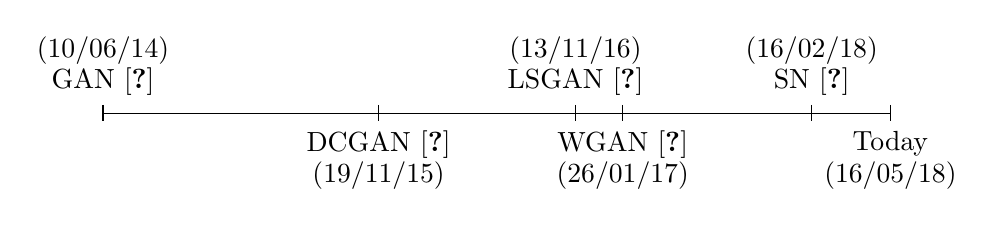
\begin{tikzpicture}
\draw (0,0) -- (10,0);

% draw vertical lines
\foreach \x in {0,3.5,6.0,6.6,9.0,10.0}
\draw (\x cm,3pt) -- (\x cm,-3pt);

% draw nodes
% 1 yr is roughly 2.5 units
\draw (0,0) node[above=3pt] {GAN \cite{goodfellow2014generative}};
\draw (0,0) node[above=14pt] {(10/06/14)};

\draw (3.5,0) node[below=3pt] {DCGAN \cite{DBLP:journals/corr/RadfordMC15}};
\draw (3.5,0) node[below=14pt] {(19/11/15)};

\draw (6,0) node[above=3pt] {LSGAN \cite{mao2017least}};
\draw (6,0) node[above=14pt] {(13/11/16)};

\draw (6.6,0) node[below=3pt] {WGAN \cite{arjovsky2017wasserstein}};
\draw (6.6,0) node[below=14pt] {(26/01/17)};

\draw (9.0,0) node[above=3pt] {SN \cite{salimans2016improved}};
\draw (9.0,0) node[above=14pt] {(16/02/18)};

\draw (10.0,0) node[below=3pt] {Today};
\draw (10.0,0) node[below=14pt] {(16/05/18)};

\end{tikzpicture}
\caption{Major contributions in the field of Generative Adversarial Networks.}
\label{fig:background-timeline}
\end{figure}


% 2014 jun 10: GAN
% 2015 nov 19: DCGAN
% 2016 nov 13: LSGAN
% 2017 jan 26: WGAN 
% 2018 feb 16: SN  
% 2018 may 16: Today 

\subsection{Generative Adversarial Networks} 
Generative Adversarial Networks (GANs) are a class of generative models trained in a adversarial manner by opposing two networks: a generative network $G$ that learns the data distribution and a discriminative network $D$ that tries and estimates the probability that a given sample came from the real training data rather than a generation from $G$. 
 
The objective for $G$ is to maximize the probability of $D$ making a mistake, and the objective for $D$ is to minimize that same probability. This framework corresponds to a minimax two-player game. In the space of arbitrary functions $G$ and $D$, a unique equilibrium solution exists, with $G$ recovering the real data distribution and $D$ equal to 0.5 everywhere, that is it's unable to distinguish the fake samples from the real ones. Since $G$ and $D$ are (de-)convolutional networks, both can be trained using available backpropagation techniques.

To learn the distribution $p_g$ over the real data $\bm{x}$, $G$ starts from sampling input variables $\bm{z}$ from a distribution of our choice $p_z(\bm{z})$, then maps the input variables $\bm{z}$ to space $G(\bm{z}; \theta_g)$ that should, after training, resemble the training data space. The discriminator, $D$, maps images to a boolean $D(\bm{x}; \theta_d)$ indicating whether images are from training data or generated from $G$. The orignal minimax objective for GANs is defined as:
\begin{equation}
\label{eq_gan}
\begin{split}
\min_G \max_D V_{\text{\tiny GAN}}(D, G) = \mathbb{E}_{\bm{x} \sim p_{\text{data}}(\bm{x})}[\log D(\bm{x})] + \mathbb{E}_{\bm{z} \sim p_{\bm{z}}(\bm{z})}[\log (1 - D(G(\bm{z})))]&.
\end{split}
\end{equation}


\subsection{Inception Score}

\subsection{Spectral Normalization}



\subsection{Least Squares Generative Adversarial Networks}
% Taken as is from LSGAN paper

Viewing the discriminator as a classifier, regular GANs adopt the sigmoid cross entropy loss function. As stated in Section \ref{sec:introduction}, when updating the generator, this loss function will cause the problem of vanishing gradients for the samples that are on the correct side of the decision boundary, but are still far from the real data. To remedy this problem, we propose the Least Squares Generative Adversarial Networks (LSGANs). Suppose we use the $a$-$b$ coding scheme for the discriminator, where $a$ and $b$ are the labels for fake data and real data,  respectively. Then the objective functions for LSGANs can be defined as follows:

\begin{equation}
\label{eq:lsgan}
\begin{split}
\min_D V_{\text{\tiny LSGAN}}(D) = &\frac{1}{2}\mathbb{E}_{\bm{x} \sim p_{\text{data}}(\bm{x})}\bigl[(D(\bm{x})-b)^2\bigr]+ \frac{1}{2}\mathbb{E}_{\bm{z} \sim p_{\bm{z}}(\bm{z})}\bigl[(D(G(\bm{z}))-a)^2\bigr] \\
\min_G V_{\text{\tiny LSGAN}}(G) = &\frac{1}{2}\mathbb{E}_{\bm{z} \sim p_{\bm{z}}(\bm{z})}\bigl[(D(G(\bm{z}))-c)^2\bigr],
\end{split}
\end{equation}


where $c$ denotes the value that $G$ wants $D$ to believe for fake data.



\subsubsection{Benefits of LSGANs}
The benefits of LSGANs can be derived from two aspects. First, unlike regular GANs, which cause almost no loss for samples that lie in a long way on the correct side of the decision boundary (Figure \ref{fig:boundary}(b)), LSGANs will penalize those samples even though they are correctly classified (Figure \ref{fig:boundary}(c)). When we update the generator, the parameters of the discriminator are fixed, i.e., the decision boundary is fixed. As a result, the penalization will make the generator to generate samples toward the decision boundary. On the other hand, the decision boundary should go across the manifold of real data for a successful GANs learning. Otherwise, the learning process will be saturated. Thus moving the generated samples toward the decision boundary leads to making them be closer to the manifold of real data. 

Second, penalizing the samples lying a long way to the decision boundary can generate more gradients when updating the generator, which in turn relieves the problem of vanishing gradients. This allows LSGANs to perform more stable during the learning process. This benefit can also be derived from another perspective: as shown in Figure \ref{fig:loss}, the least squares loss function is flat only at one point, while the sigmoid cross entropy loss function will saturate when $x$ is relatively large.




\section{Approach}
%
%Describe the final approach you are take for this problem.
%For instance, here you would describe the details of the network’s
%architecture. What training parameters and techniques you have used.
%The computational complexity of your model. And similar questions.
%To help explain your approach please make figures to accompany your
%text description. (1-3 pages)
For our research we replicated the DCGAN network, described in great detail in \cite{DBLP:journals/corr/RadfordMC15}, in Tensorflow using Taehoon Kim's (found \href{https://github.com/carpedm20/DCGAN-tensorflow}{here}) implementation as inspiration.

\subsection{Architecture}

\paragraph{Generator architecture details.} The generator's architecture is depicted in Figure \ref{fig:architecture}. The input layer is a vector of size 100 followed by 4 convolutional hidden layers. The output layer is then the picture generated that feeds into the discriminator. The 4 hidden layers use the ReLU activation function while the output layer uses the $\tanh$ function. The authors of DCGAN state that using a bounded activation like $\tanh$ for the output layer allowed the network to \textit{``learn more quickly to saturate and cover the color space of the training distribution"} \cite{DBLP:journals/corr/RadfordMC15} (p. 3).
\paragraph{Discriminator architecture details.} The discriminator's architecture follows a very similar structure with the obvious exception of the input and output layers. The input layer for the discriminator consists of an image, while the output layer is a single neuron activated by a $sigmoid$ function that represents the classification of real vs fake images. The convolutional layers use the leaky ReLU activation function.\begin{figure}[h]
\centering
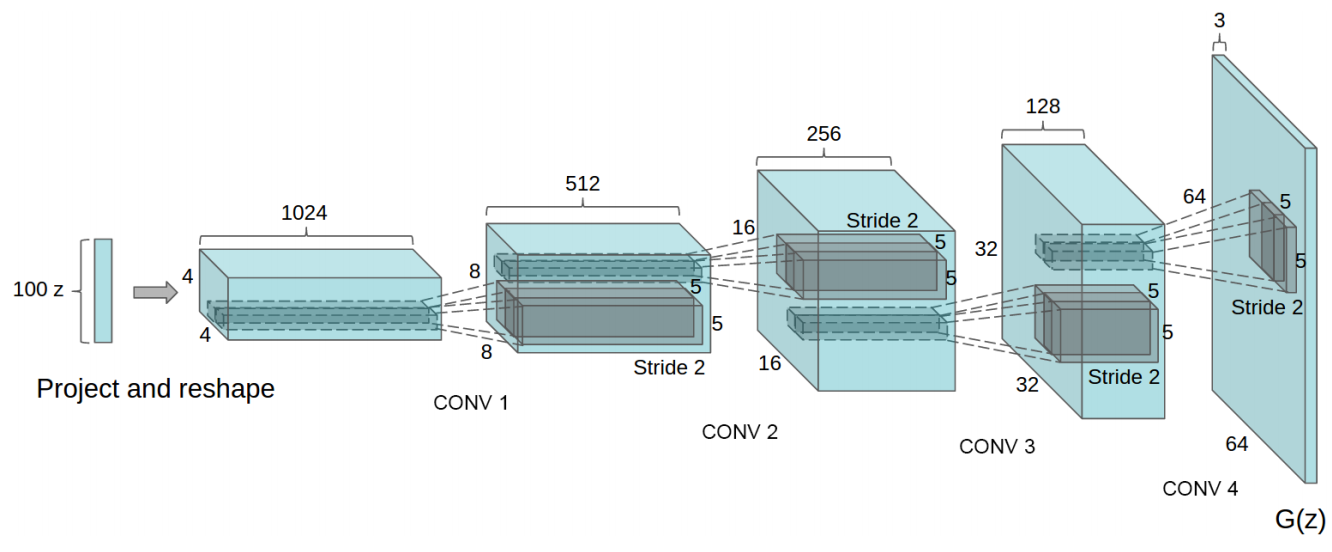
\includegraphics[width=0.7\textwidth]{figures/DCGAN.png}
\caption{Generator Network architecture. Cited from \cite{DBLP:journals/corr/RadfordMC15} }
\label{fig:architecture}
\end{figure}

\subsection{Training}
We train all networks using the Adam optimizer \cite{2014arXiv1412.6980K} with a learning rate of 0.002 and a $\beta_1$ value (exponential decay rate of first moment estimate) of 0.5, as advised by the authors of DCGAN.

Due to the complexity of the networks, we run all of our experiments on two separate GPU enabled devices. We run most of our experiments on a laptop equipped with a NVIDIA GTX 1060 GPU while some training iterations were done using a Amazon Web Service EC2 Deep Learning instance with a NVIDIA K80 GPU. Even though using these machines makes our training much faster, each training iteration takes a considerable amount of time. This results in us having to run our experiments over night and use the days to implement our networks and interpret the results. 

\subsection{Data Collection}
%not sure if this is actually something we want to include and if so where it should be introduced so feel free to change it
%TODO possibly add a reference instead of the hyperlink

During experimentation we mostly rely on the popular benchmark dataset \href{https://www.cs.toronto.edu/~kriz/cifar.html}{CIFAR10}, however an additional dataset was collected using \href{https://www.flickr.com/services/api/}{Flickr's API}. Due to varying amounts of quality pictures of objects that would be interesting to base the image generation on, a collection that included mostly different reptiles with a fair amount of arachnid's thrown into the mix was ultimately settled upon, this dataset will be referred to as the Reptiles dataset from here on. In total the data set is made up of approximately 20K color images, all re-sized to dimensions of 108x108x3 before training was conducted. Examples of images can be seen in figure \ref{fig:reptiles}.%
\begin{figure}[H]
\centering
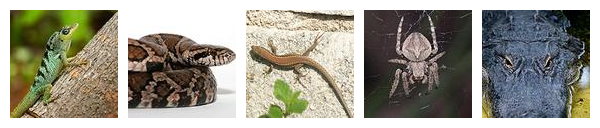
\includegraphics[width=0.7\textwidth]{figures/reptiles.png}
\caption{Examples from the Reptiles data set}
\label{fig:reptiles}
\end{figure}

\section{Experiments}
%In this section, you should
%present the results you achieved with various experiments. The results
%can be presented in tables, plots, etc. 
The project consists of 8 distinct experiments where each experiment varies from the others either based on what dataset is used or what network settings are used.

\subsection{Inception Score Considerations}

We present a challenge related to the computation and evaluation of the inception score. Most authors evaluate the inception score on 50K GAN-generated images, as recommend by the authors of the original paper \cite{salimans2016improved}. By running a few preliminary experiments, we quickly realized that on top of the actual training of the network, sampling and computing the inception score are also resource-intensive tasks, and sampling 50K images is simply not possible with the time or resources available for this project.


Now, the number of images considered for evaluating the inception score has an impact on this score, as Table \ref{table:exp-isc} depicts. This is due to the fact that the inception score not only evaluates the content of a given image but also the distribution of categories among the whole set of images resulting from the split. In other words, the score is sensitive to the number of images divided by the number of splits. 

\begin{table}[H]
\centering
\setlength{\tabcolsep}{0.5em} % for the horizontal padding

\begin{subtable}{.5\textwidth}
\centering

\begin{tabular}{l l l}
\toprule
Images & Splits & Inception score  \\ 
\midrule
      256  & 5 & 8.13 +- 0.41 \\   
      512  & 5 & 8.04 +- 0.54 \\ 
      1024 & 5 & 9.79 +- 0.36 \\
\bottomrule
\end{tabular}

\end{subtable}% <---- don't forget this %
\begin{subtable}{.5\textwidth}
\centering

\begin{tabular}{l l l}
\toprule
Images & Splits & Inception score  \\ 
\midrule
      256  & 10 & 6.72 +- 0.55 \\   
      512  & 10 & 7.92 +- 0.56\\ 
      1024 & 10 & 8.95 +- 0.44 \\
\bottomrule
\end{tabular}
\end{subtable}%
%
\vspace{0.3cm}
\caption{Inception score for various number of samples of the cifar10 dataset.}
\label{table:exp-isc}
\end{table}%
We choose to stick with 1024 generated images and 5 splits for all of our experiments. With this configuration, we have a target inception score of 9.79. As expected, this is below the claimed inception score of the whole cifar10 dataset, 11.24 \cite{salimans2016improved}. Thus we won't reach state of the art results in terms of inception score, but this isn't an issue since our purpose is to compare various improvements of GAN networks, which isn't affected by this choice. We applied the same calculations to our Reptile data set, resulting in a target inception score of $10.2415905 +- 0.92625165$. Other considerations on the inception score are explained in \cite{barratt2018note}.

\subsection{DCGAN}
\label{sec:exp-dcgan}

We implement our baseline model in this section. The DCGAN is evaluated on cifar10. We present the evolution of the inception score in Figure \ref{fig:exp-dcgan-is} and both losses in Figure \ref{fig:exp-dcgan-losses}. These results serve as a reference for all our other experiments. The inception score seems to plateau around 5.8 with considerable deviations. Both the D and G losses are very unstable during training. \\
It is however important to note that losses can hardly be interpreted when treating with GANs, since the generator and discriminator are in a situation of competition where an improvement on the one leads to a deterioration on the other.
\begin{figure}[H]
    \centering
    \begin{subfigure}[t]{0.49\textwidth}
        \centering
		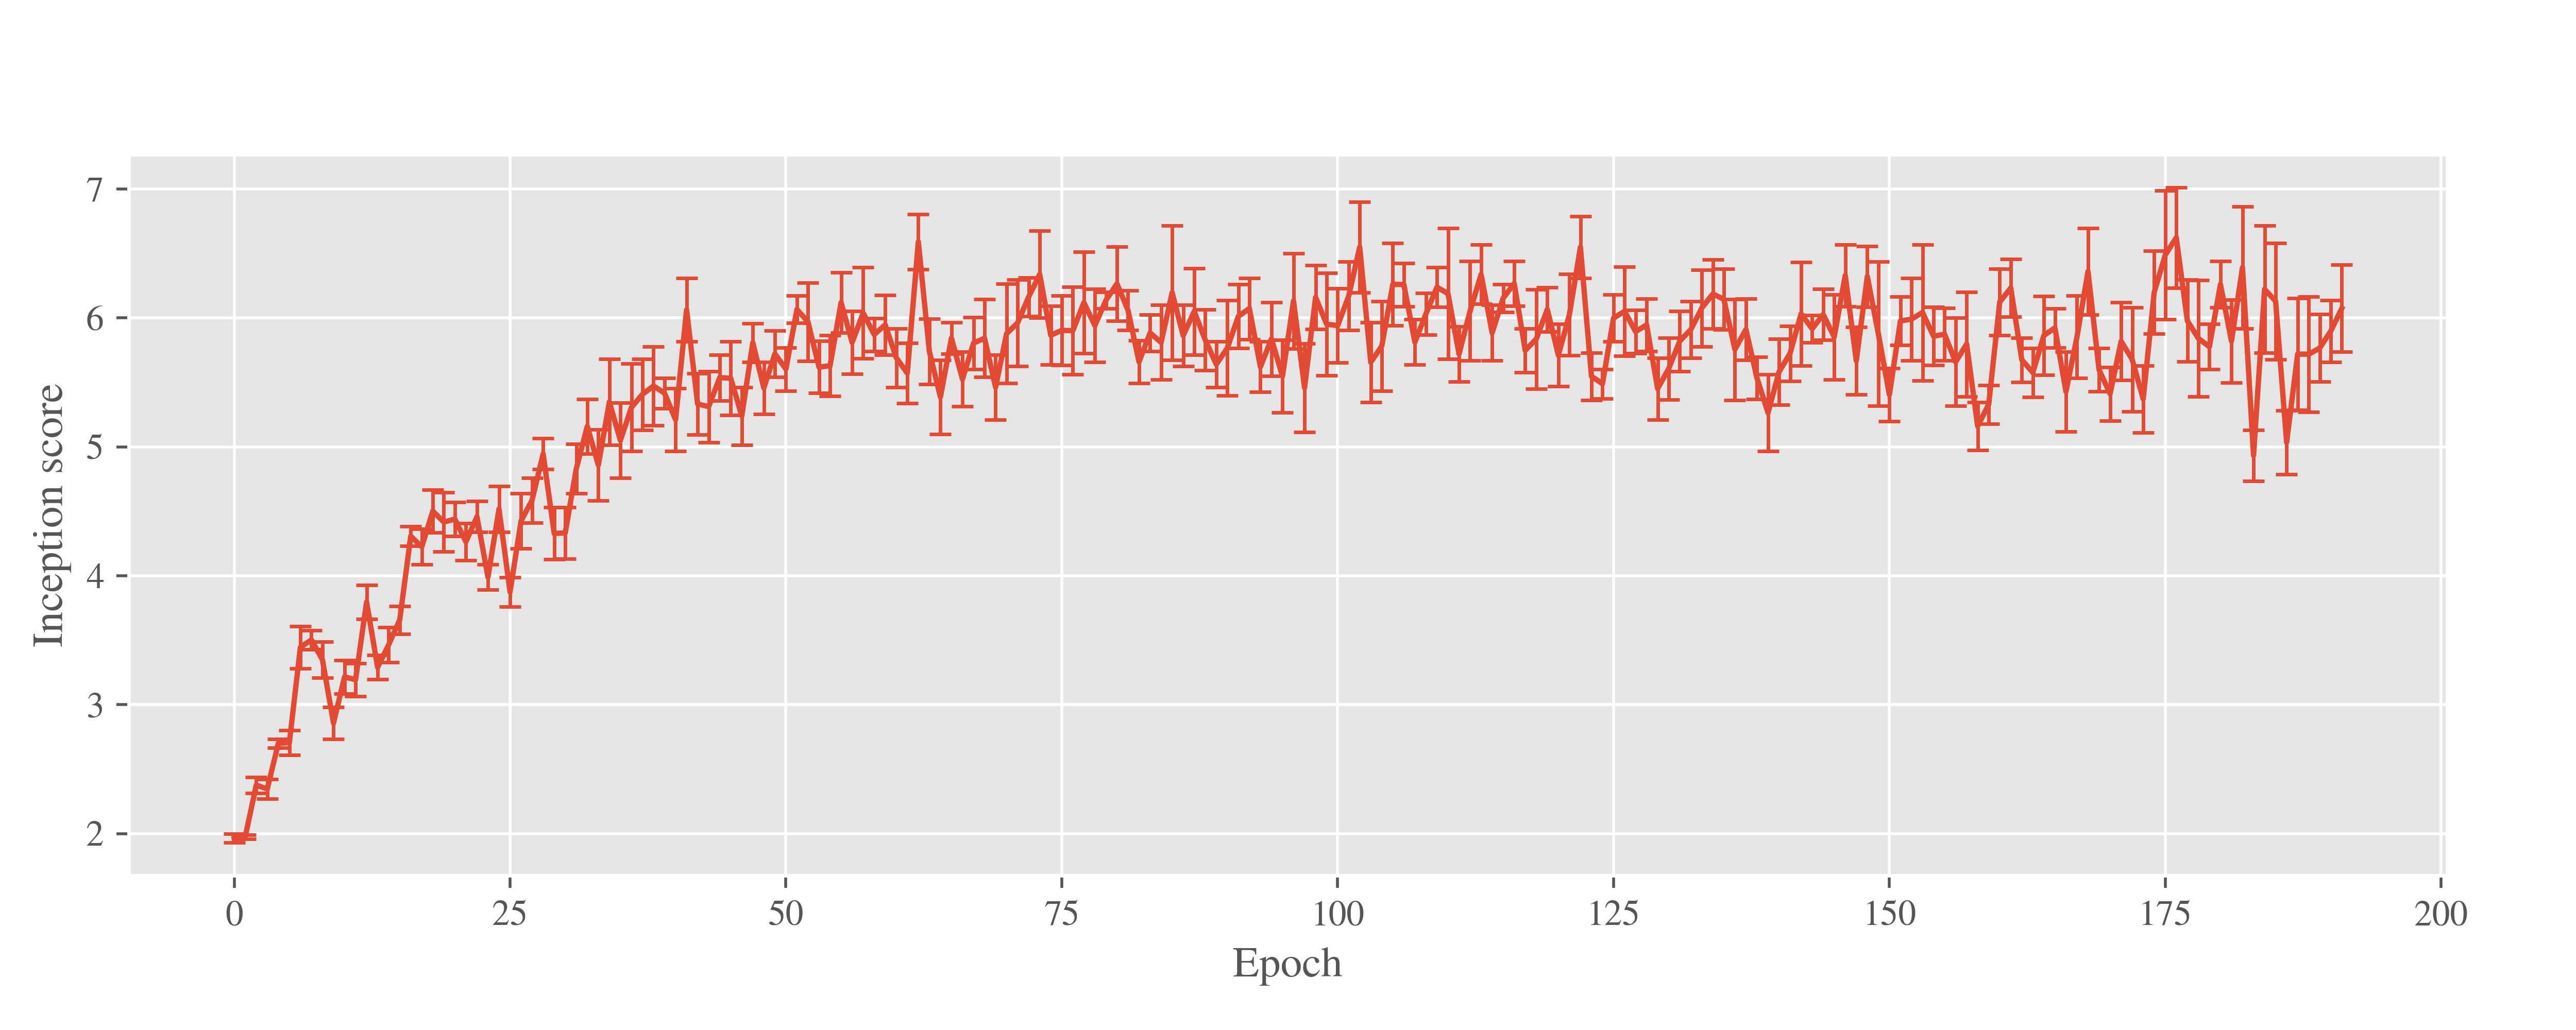
\includegraphics[width=\textwidth]{../code/results/figures/dcgan_cifar10_is.png}
		\caption{Inception score}
		\label{fig:exp-dcgan-is}
    \end{subfigure}
    \begin{subfigure}[t]{0.49\textwidth}
        \centering
        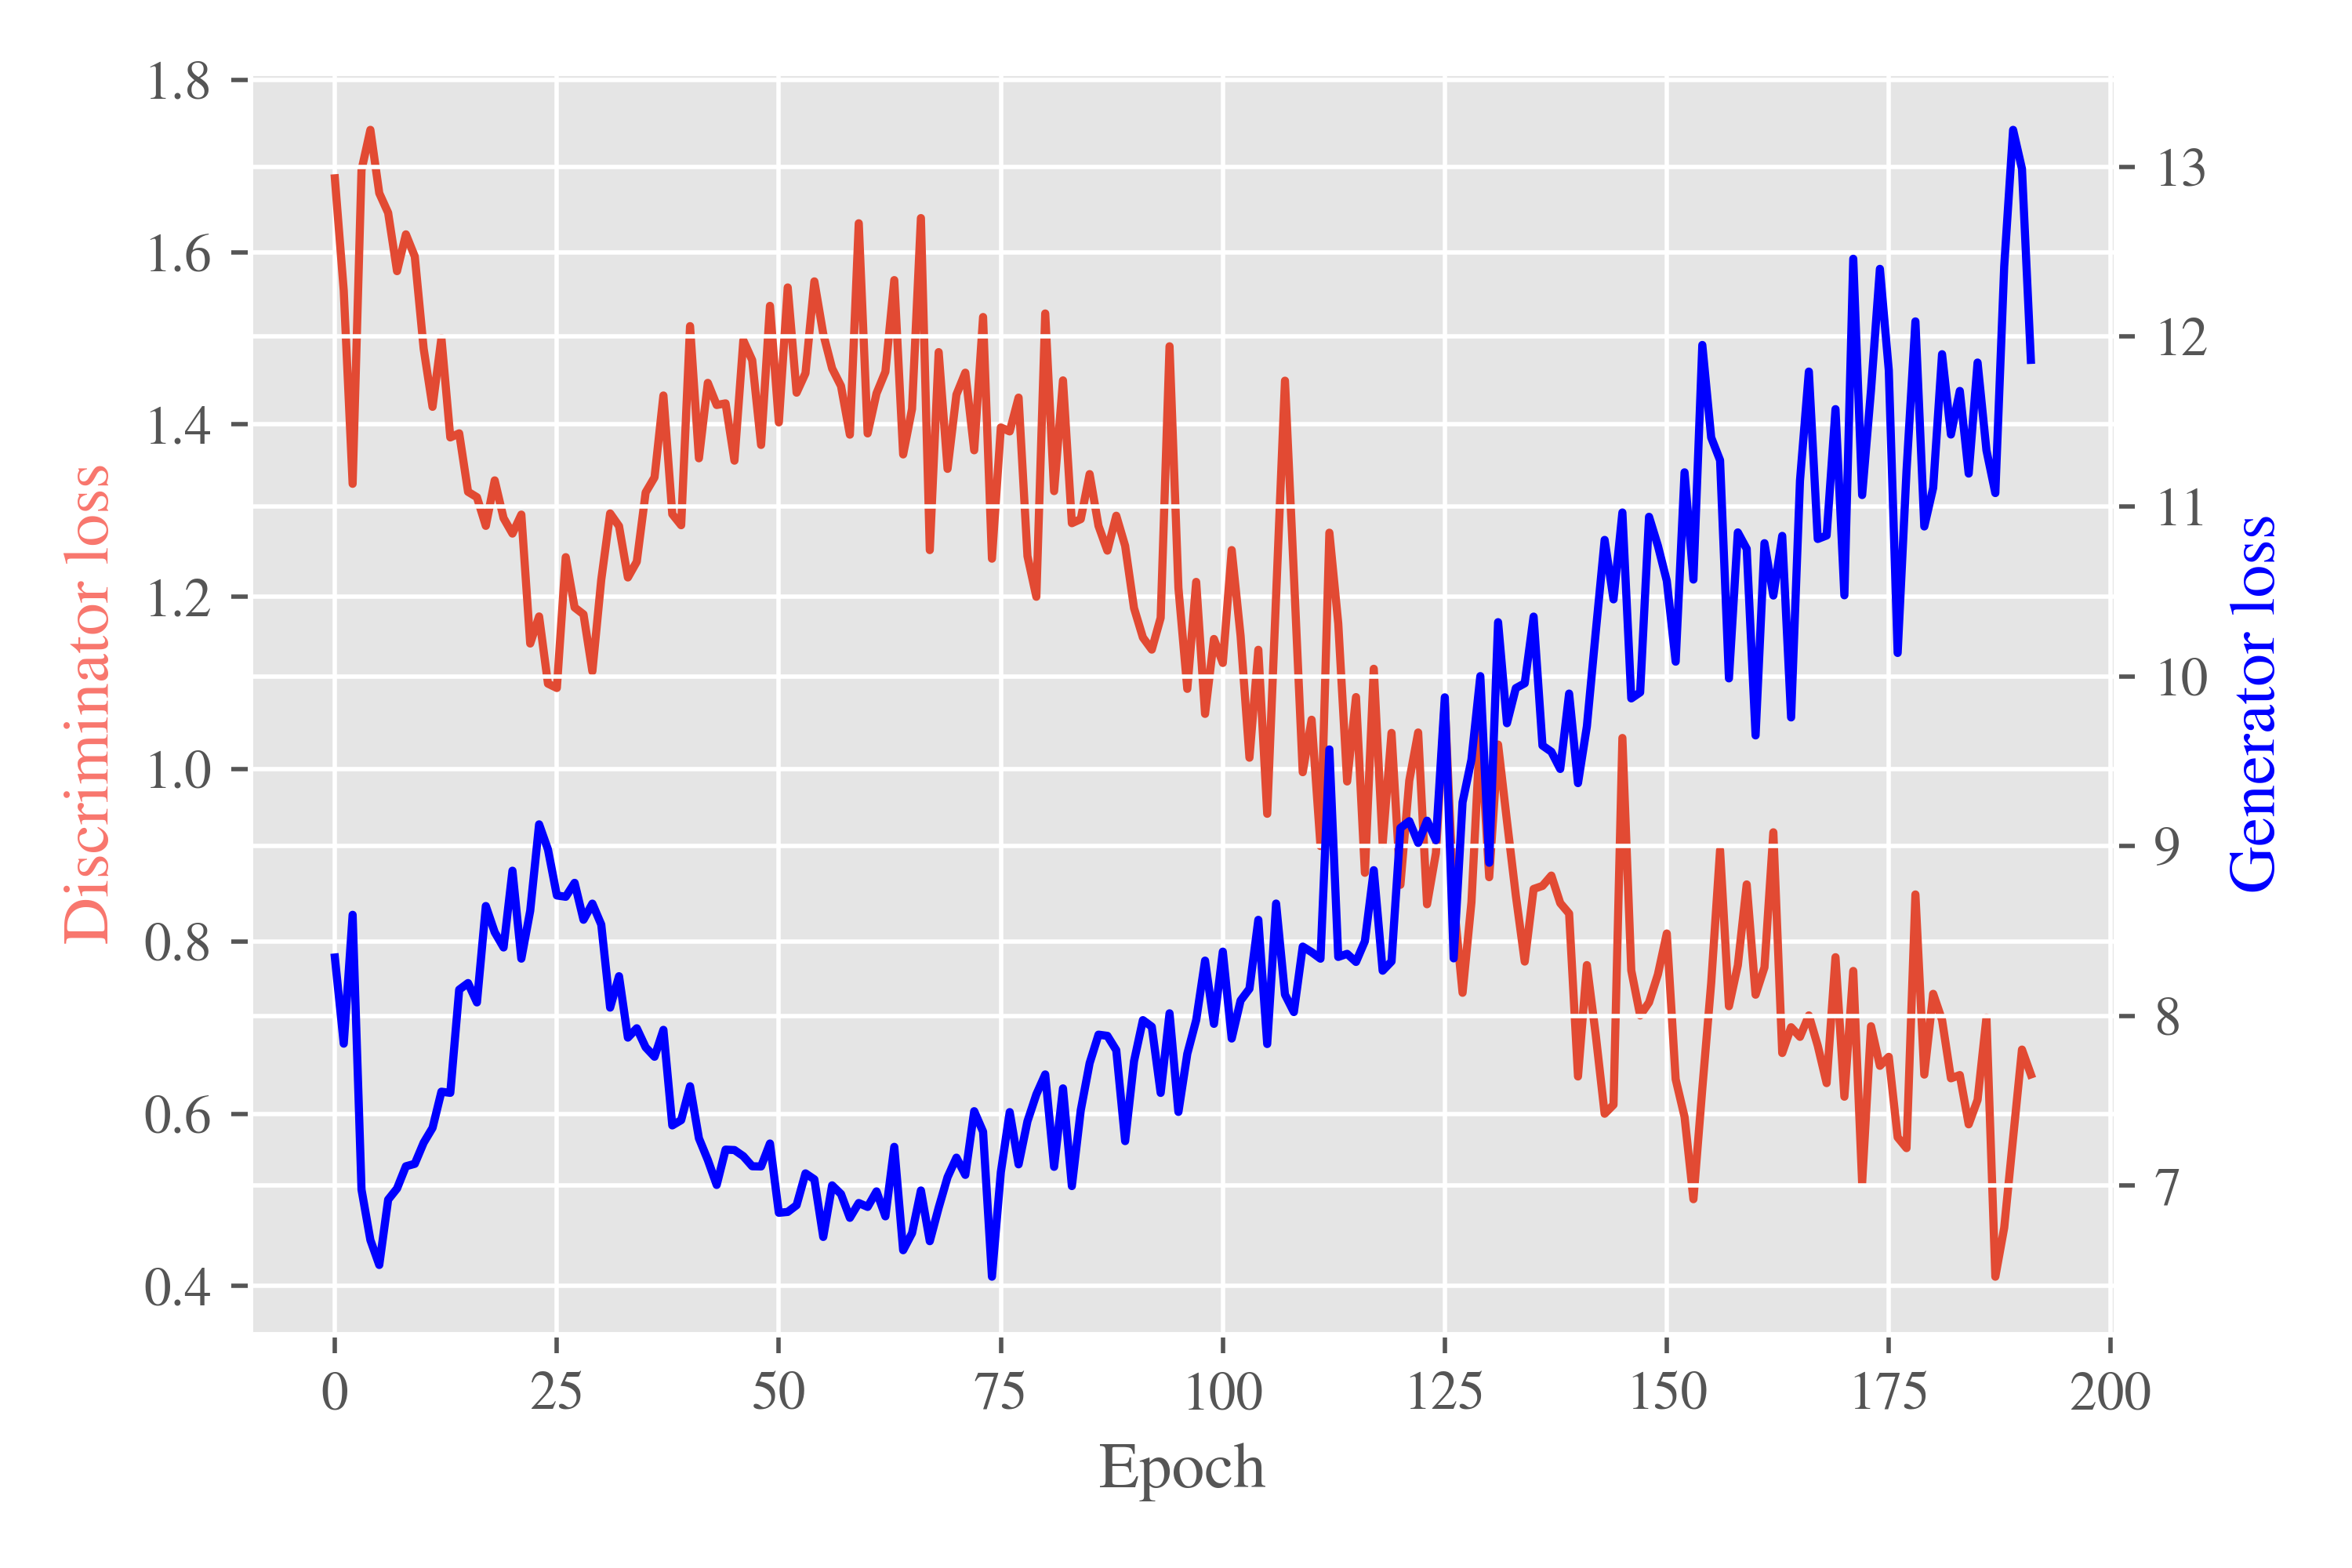
\includegraphics[width=\textwidth]{../code/results/figures/dcgan_cifar10_losses.png}
		\caption{Losses}
		\label{fig:exp-dcgan-losses}
    \end{subfigure}
    \caption{DCGAN - training on CIFAR10 over 190 epochs.}
\end{figure}
We conduct a visual inspection of the generated images and observe that many of them look alike, if not identical. This is a common phenomenon called mode collapse, in which the generator fails to learn the complete multimodal structure of the target data distribution and rather learns a subset of modes, allowing it to trick the discriminator but not to reproduce the target data distribution.
\subsection{SN-DCGAN}
\label{sec:exp-sndcgan}
We implement the spectral normalization layer and use on the discriminator of the DCGAN used in the previous section. We present the evolution of the inception score and losses in Figures \ref{fig:exp-sndcgan-is} and \ref{fig:exp-sndcgan-losses}, respectively.
   
% is
\begin{figure}[h]
\centering
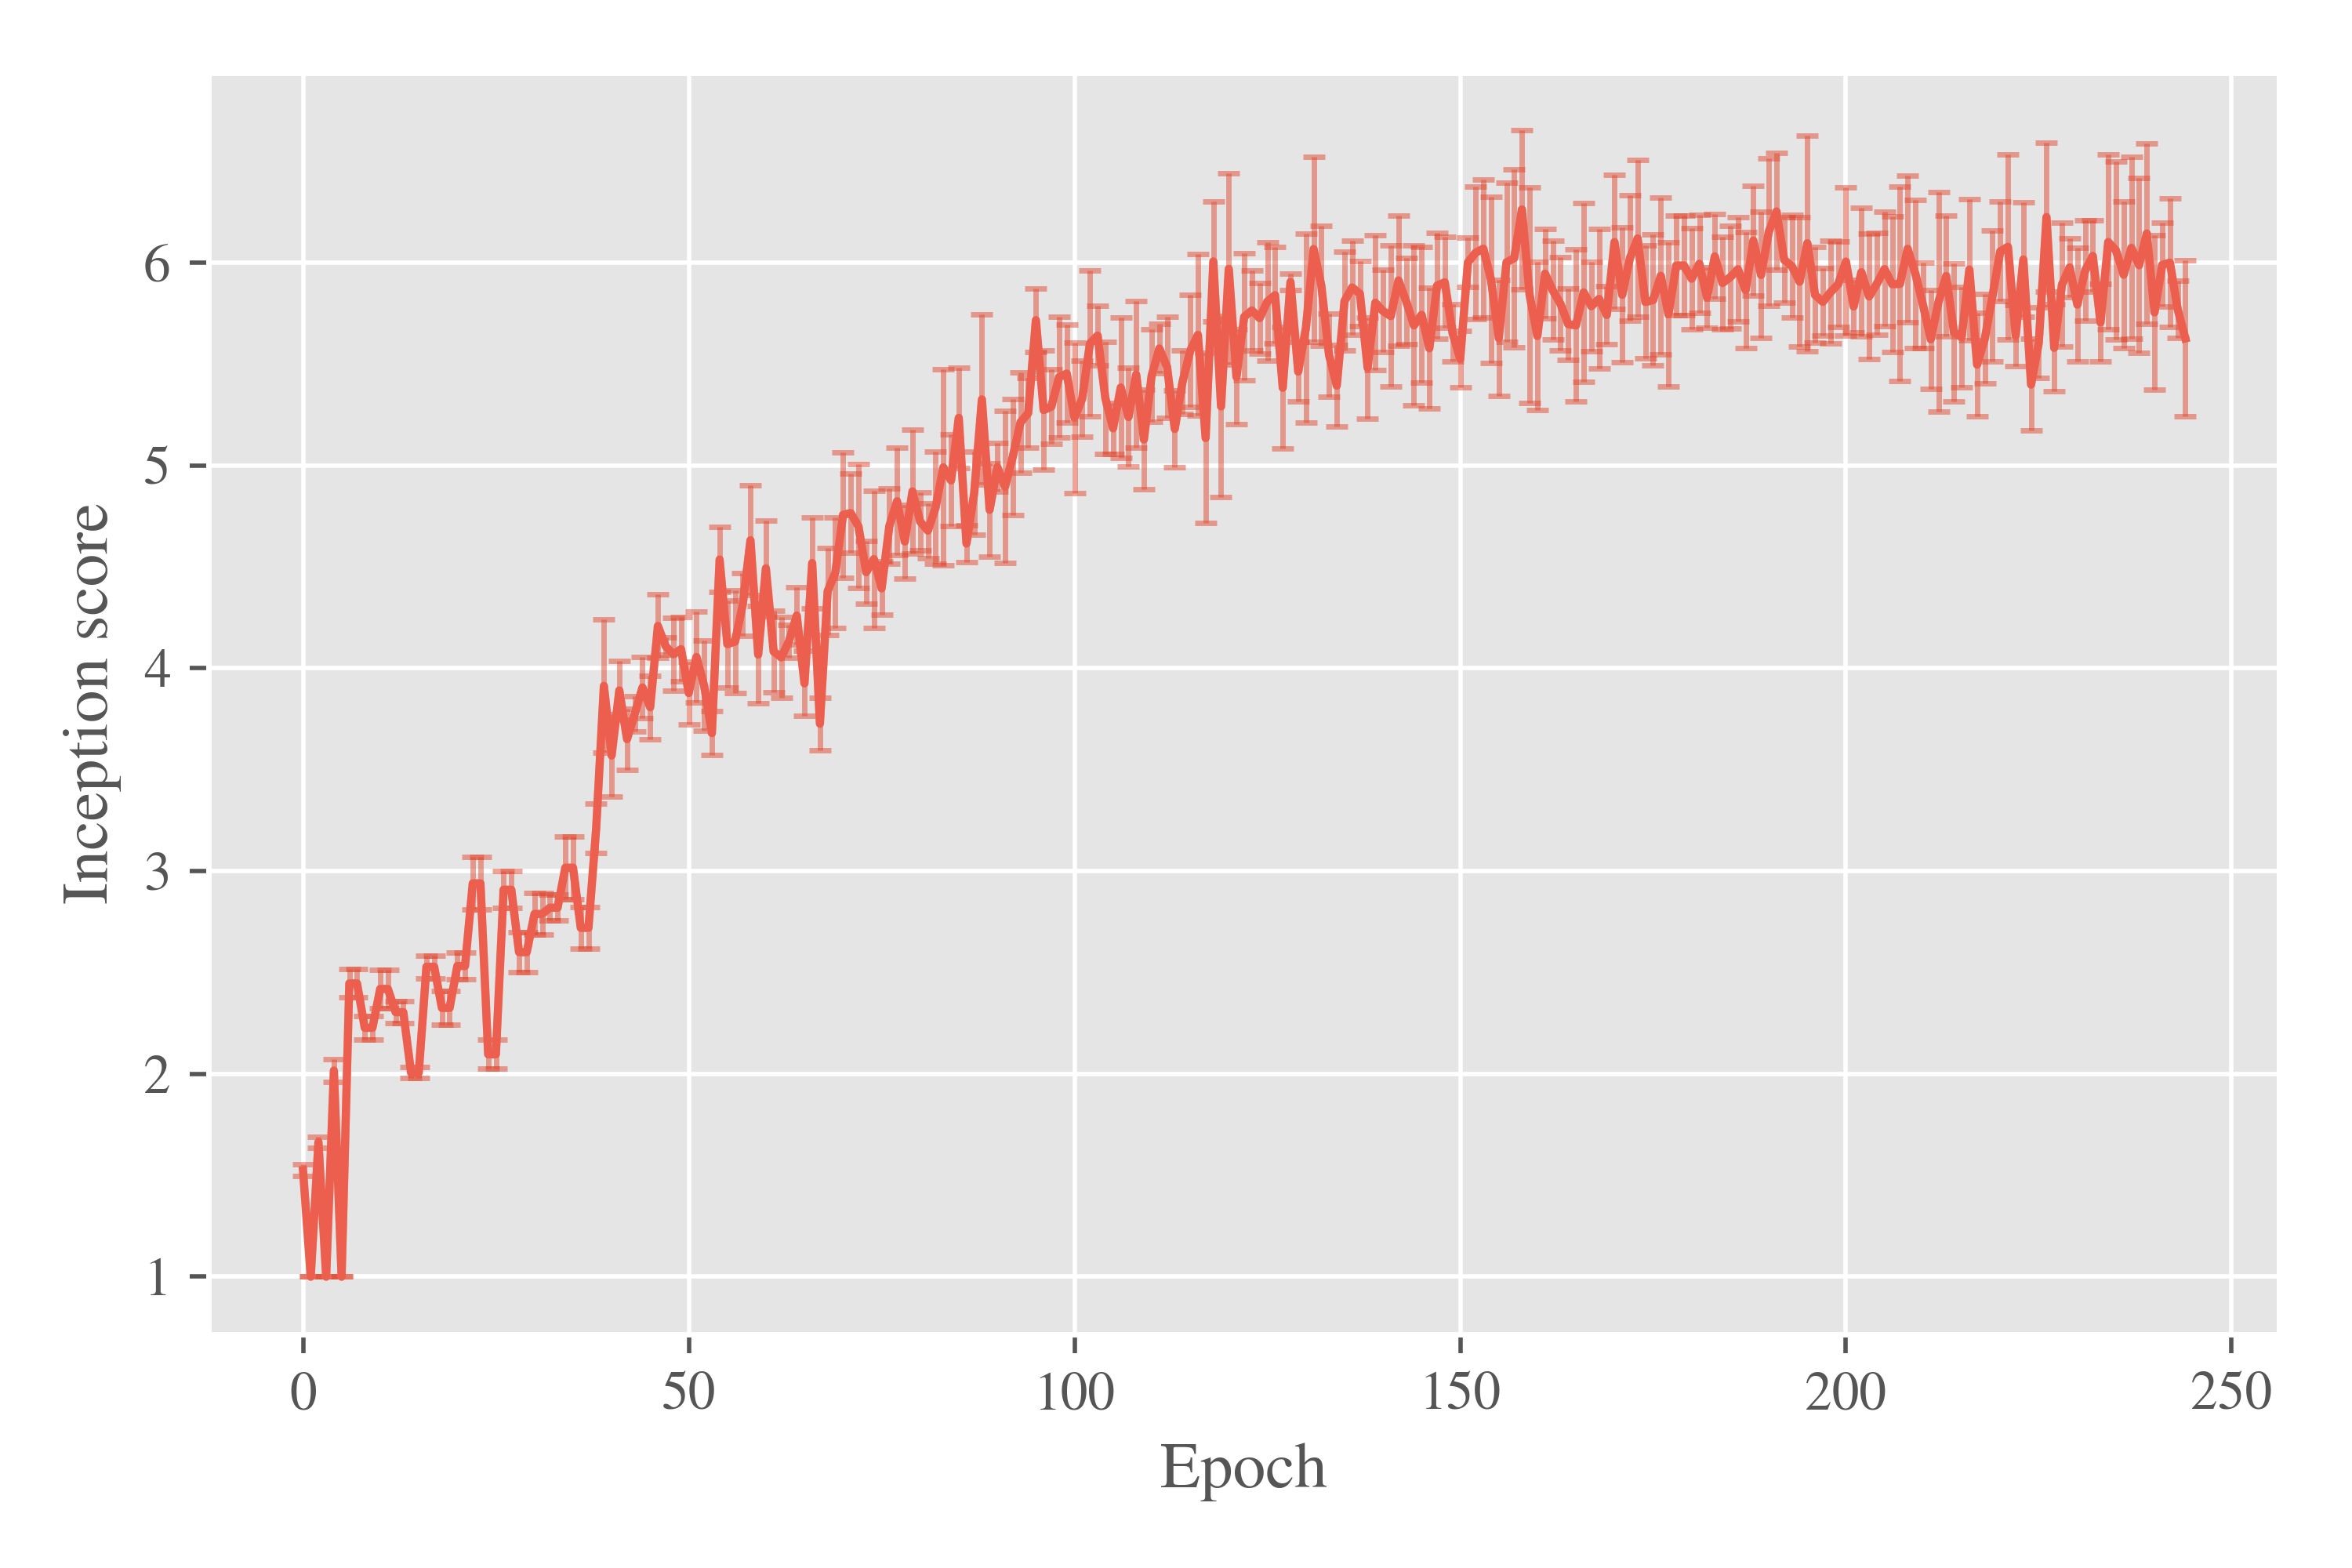
\includegraphics[width=\textwidth]{../code/results/figures/sndcgan_cifar10_is.png}
\caption{SN-DCGAN - Inception score, training on cifar10 over ~250 epochs}
\label{fig:exp-sndcgan-is}
\end{figure}
We don't notice any significant improvement on the mean of the inception score after convergence. However, the average standard deviation is reduced compared to that of the DCGAN without spectral normalization, depicted in Figure \ref{fig:exp-dcgan-is}.
% losses
\begin{figure}[h]
\centering
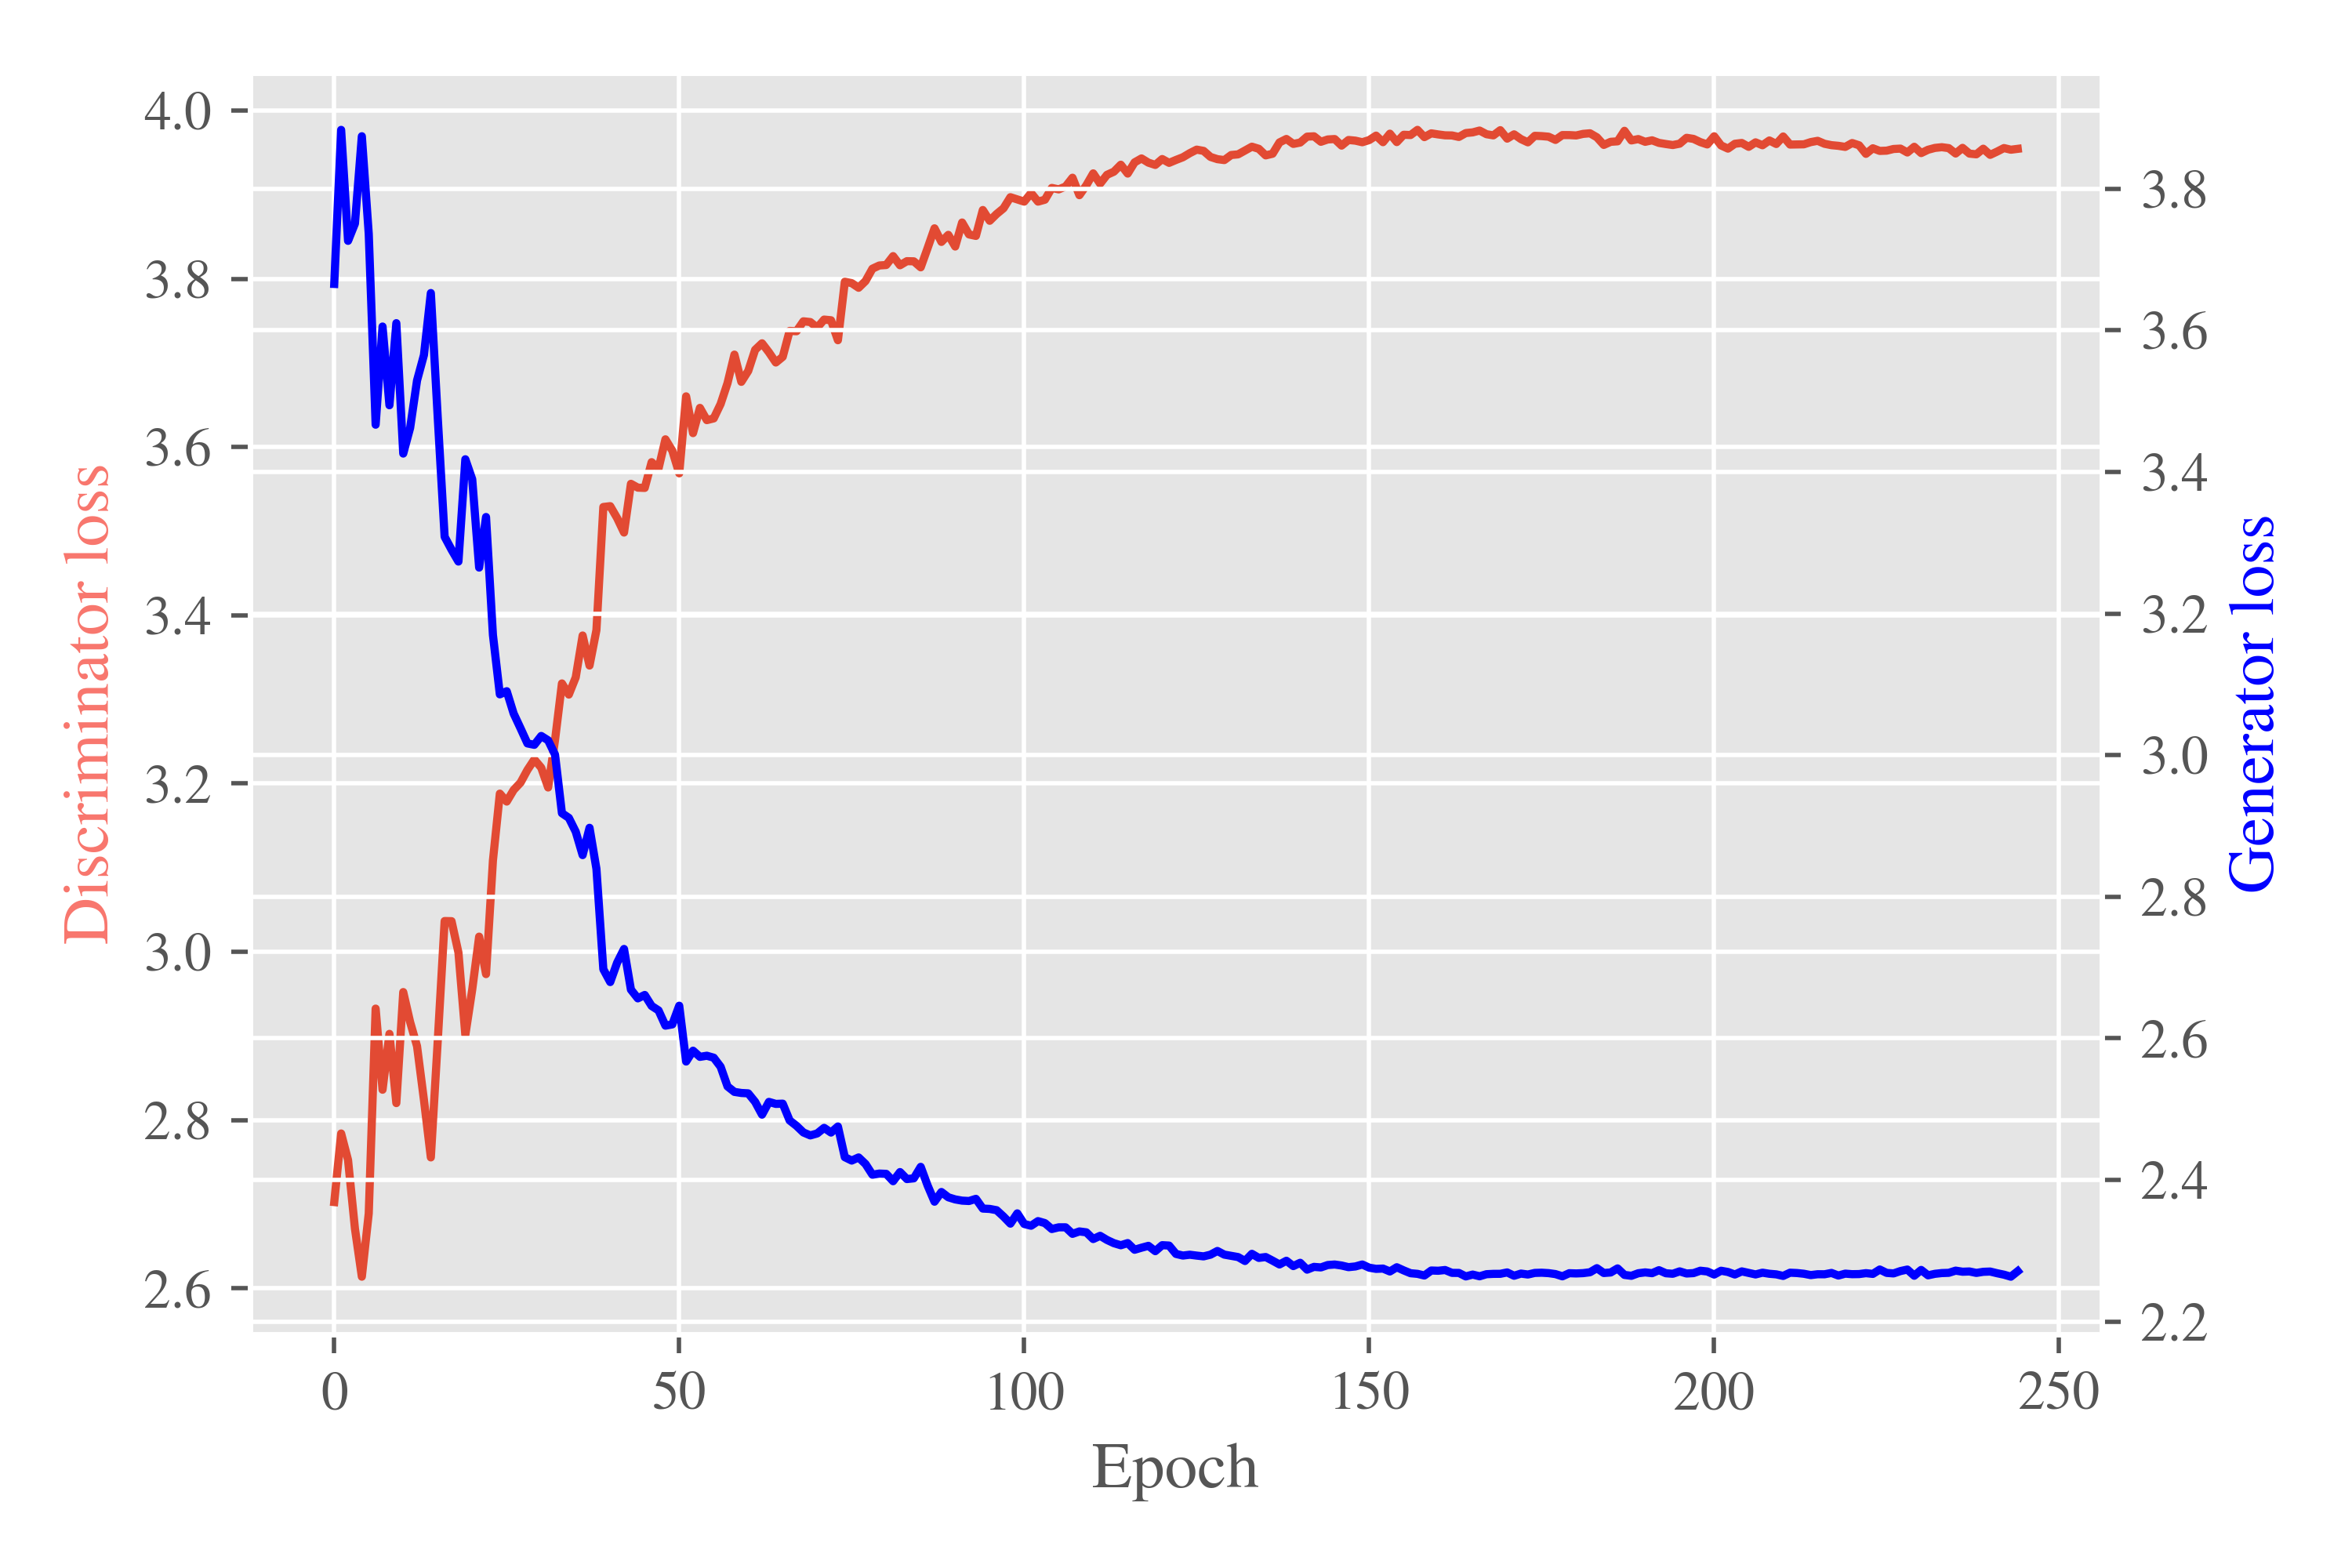
\includegraphics[width=\textwidth]{../code/results/figures/sndcgan_cifar10_losses.png}
\caption{SN-DCGAN - Losses training on cifar10 over ~250 epochs.}
\label{fig:exp-sndcgan-losses}
\end{figure}
In Figure \ref{fig:exp-dcgan-losses}, we observe that both losses are much smoother with spectral normalization. This is the desired result; the original intent of the paper on spectral normalization was to provide a solution to stabilize the training of GANs \cite{miyato2018spectral}. 
\subsection{W-DCGAN}
\label{sec:exp-w-dcgan}
We present the evolution of the Inception score and losses in Figures \ref{fig:exp-w-dcgan-is} and \ref{fig:exp-w-dcgan-losses}, respectively. We did not expect to a get good performance using this setup since we did not implement any method enforcing the Lipschitz continuity of the discriminator functions, which is required by WGAN. These results coincide with our expectations.
   
\begin{figure}[H]
    \centering
    \begin{subfigure}[t]{0.49\textwidth}
        \centering
		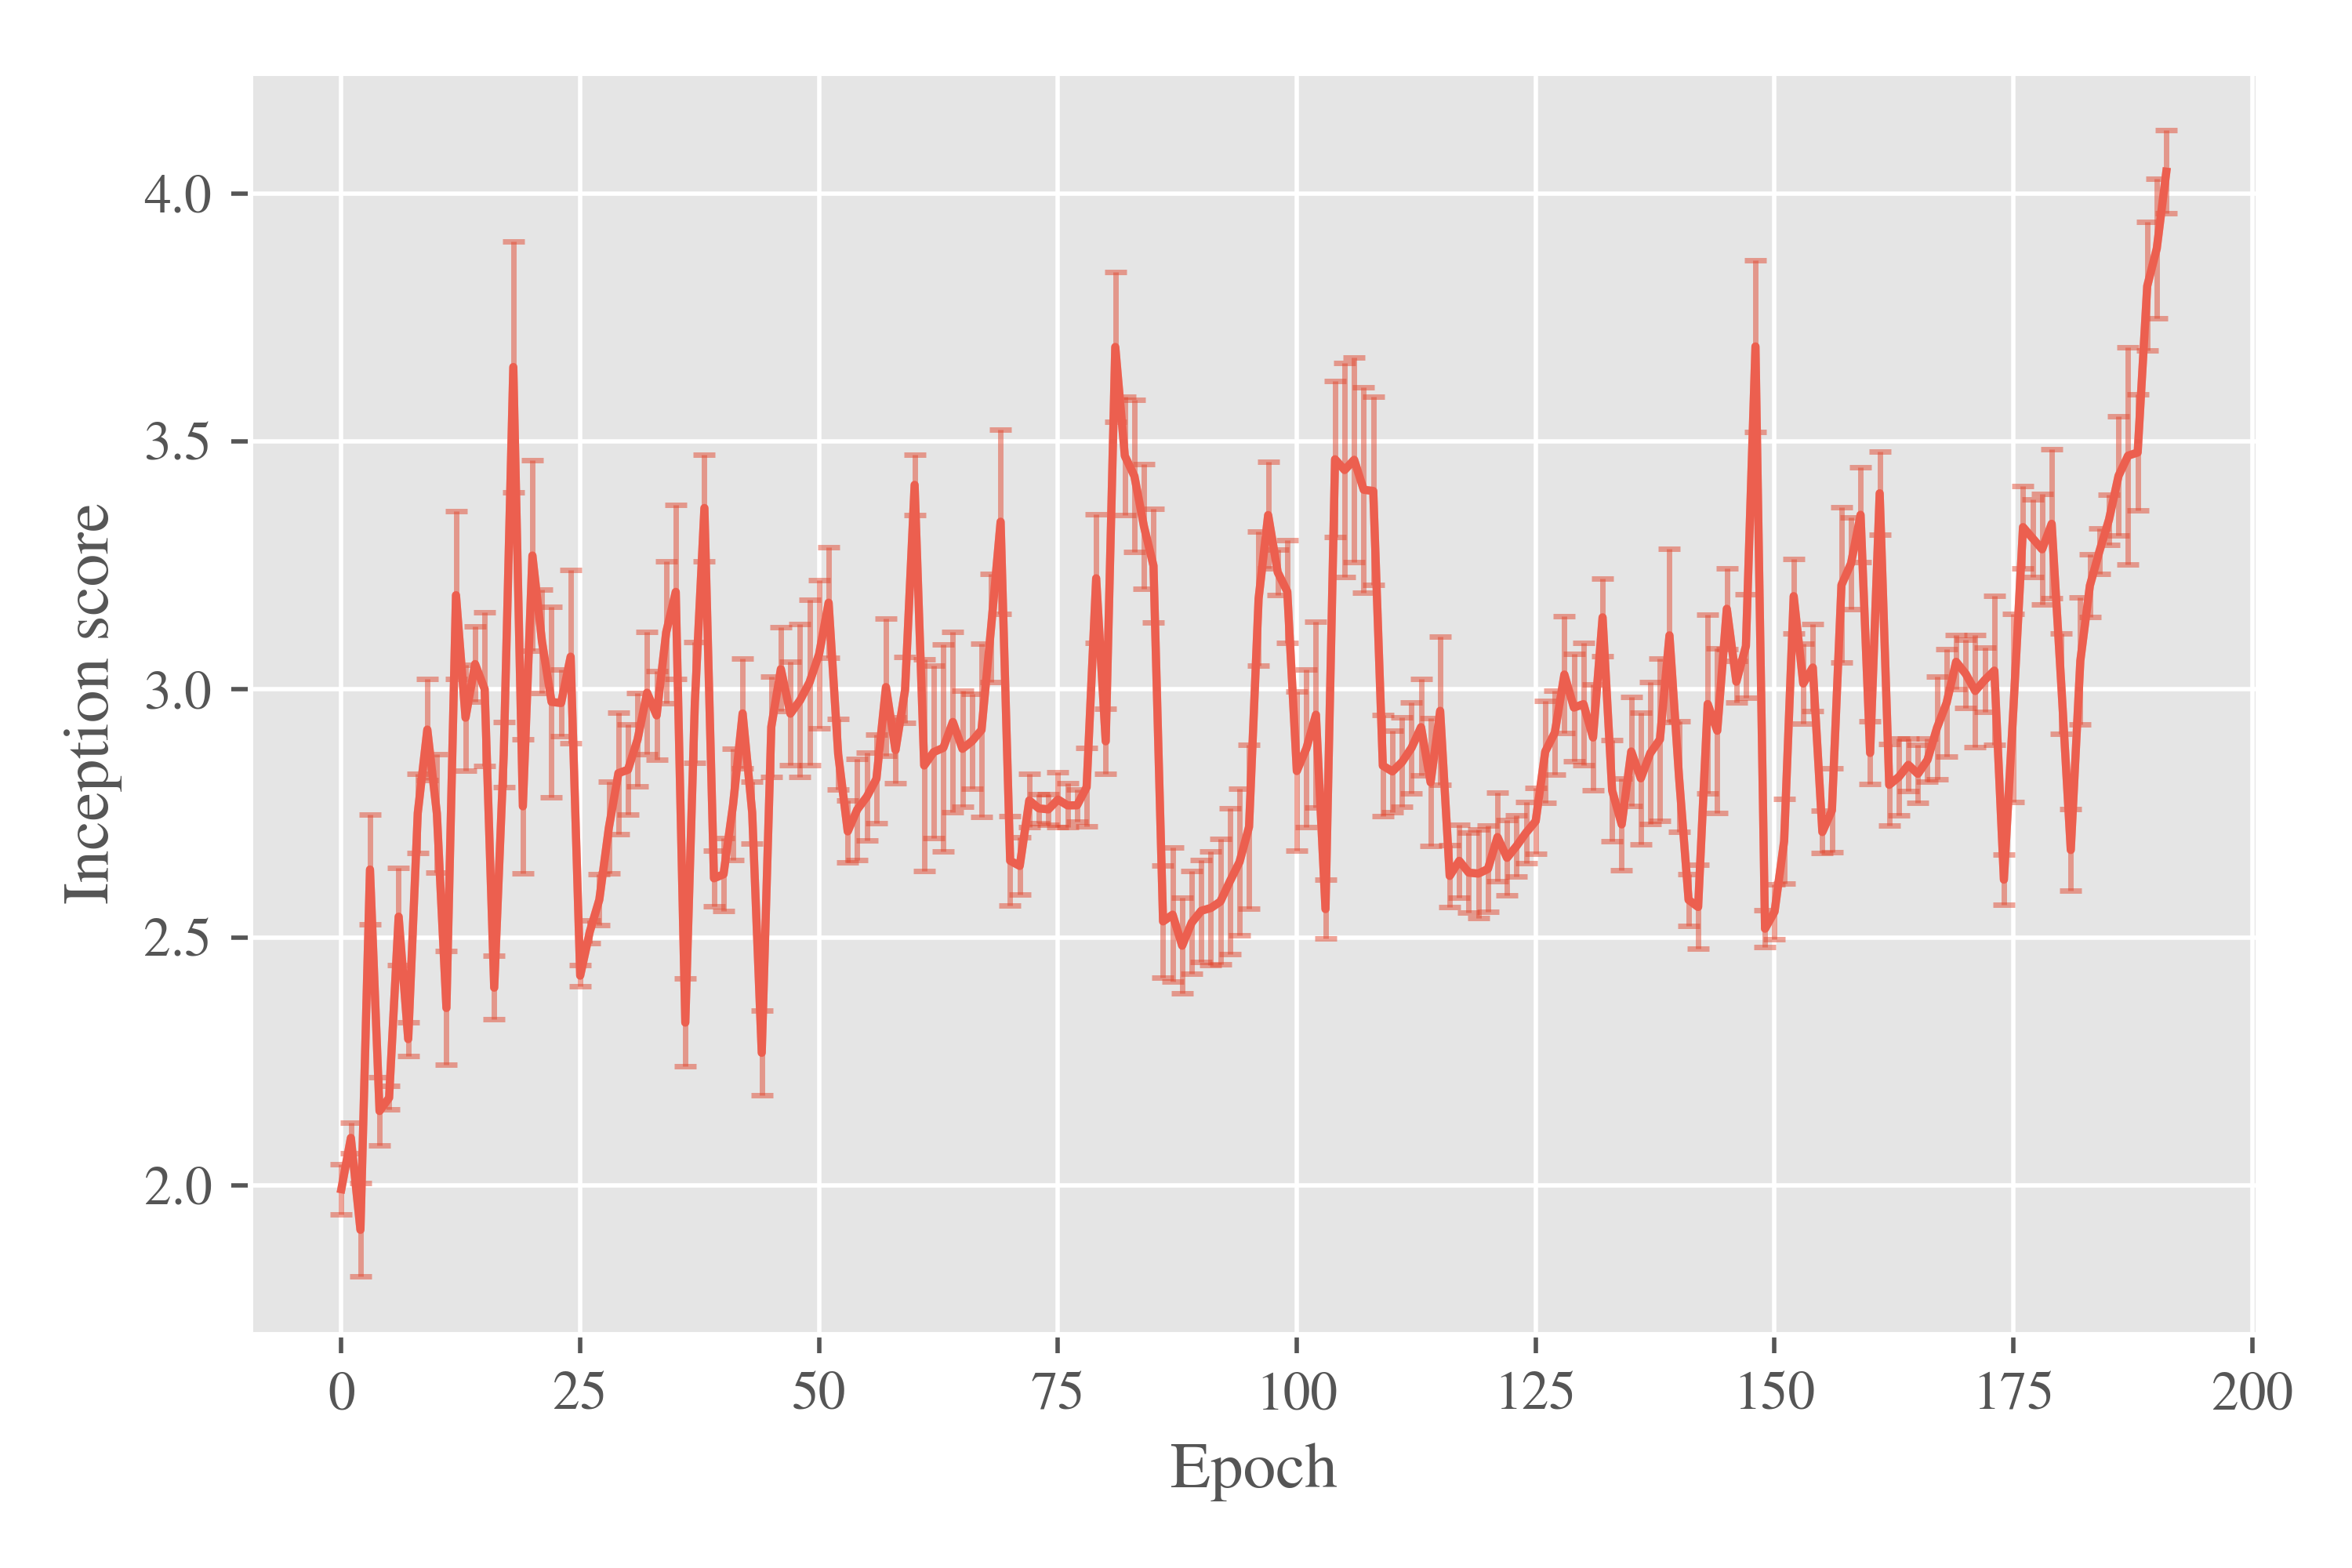
\includegraphics[width=\textwidth]{../code/results/figures/w-dcgan_cifar10_is.png}
		\caption{Inception score\\~}
		\label{fig:exp-w-dcgan-is}
    \end{subfigure}
    \begin{subfigure}[t]{0.49\textwidth}
        \centering
        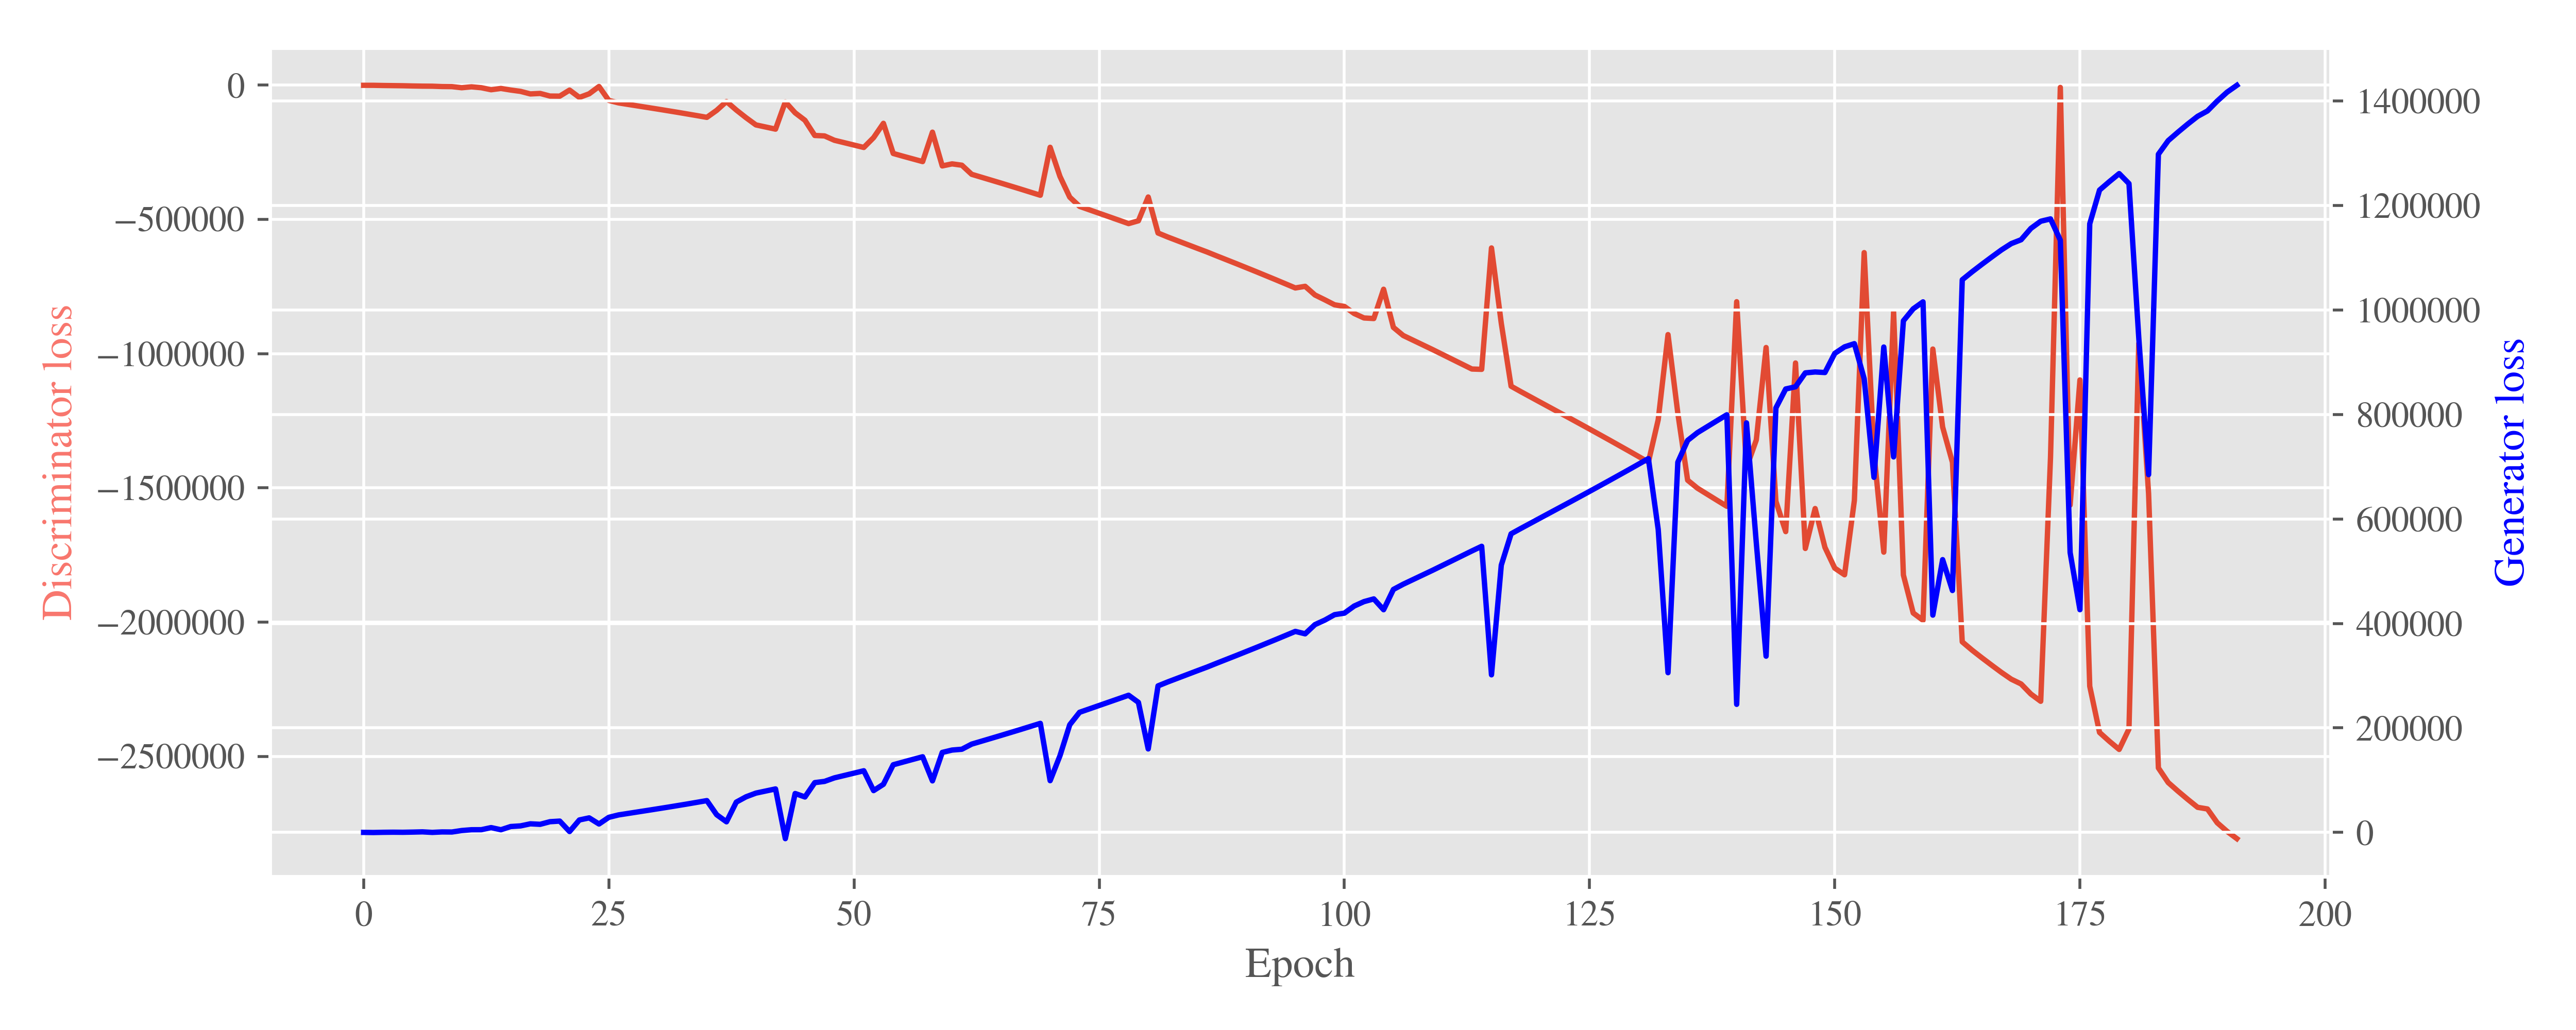
\includegraphics[width=\textwidth]{../code/results/figures/w-dcgan_cifar10_losses.png}
		\caption{Losses\\~}
		\label{fig:exp-w-dcgan-losses}
    \end{subfigure}
    \caption{W-DCGAN - training on CIFAR10 over 200 epochs.}
\end{figure}

%We observe that both losses are much smoother with spectral normalization. This is the desired result; the original intent of the paper on spectral normalization was to provide a solution to stabilize the training of GANs \cite{miyato2018spectral}. By visual inspection of the generated images we observe a significant reduce in mode collapse and a noticeable improvement of image quality. This did however not result in a significant Inception score improvement.
\subsection{W-WC-DCGAN}
\label{sec:exp-w-wc-dcgan}
We implement weight clipping (WC) on top of the W-DCGAN from the previous section. As stated before, the authors of WGAN state that this method is a far from ideal way to ensure a norm on the gradients. However, we still expect it to outperform the W-DCGAN. We present the evolution of the Inception score and losses in Figures \ref{fig:exp-w-wc-dcgan-is} and \ref{fig:exp-w-wc-dcgan-losses}, respectively. %
\begin{figure}[H]
    \centering
    \begin{subfigure}[t]{0.49\textwidth}
        \centering
		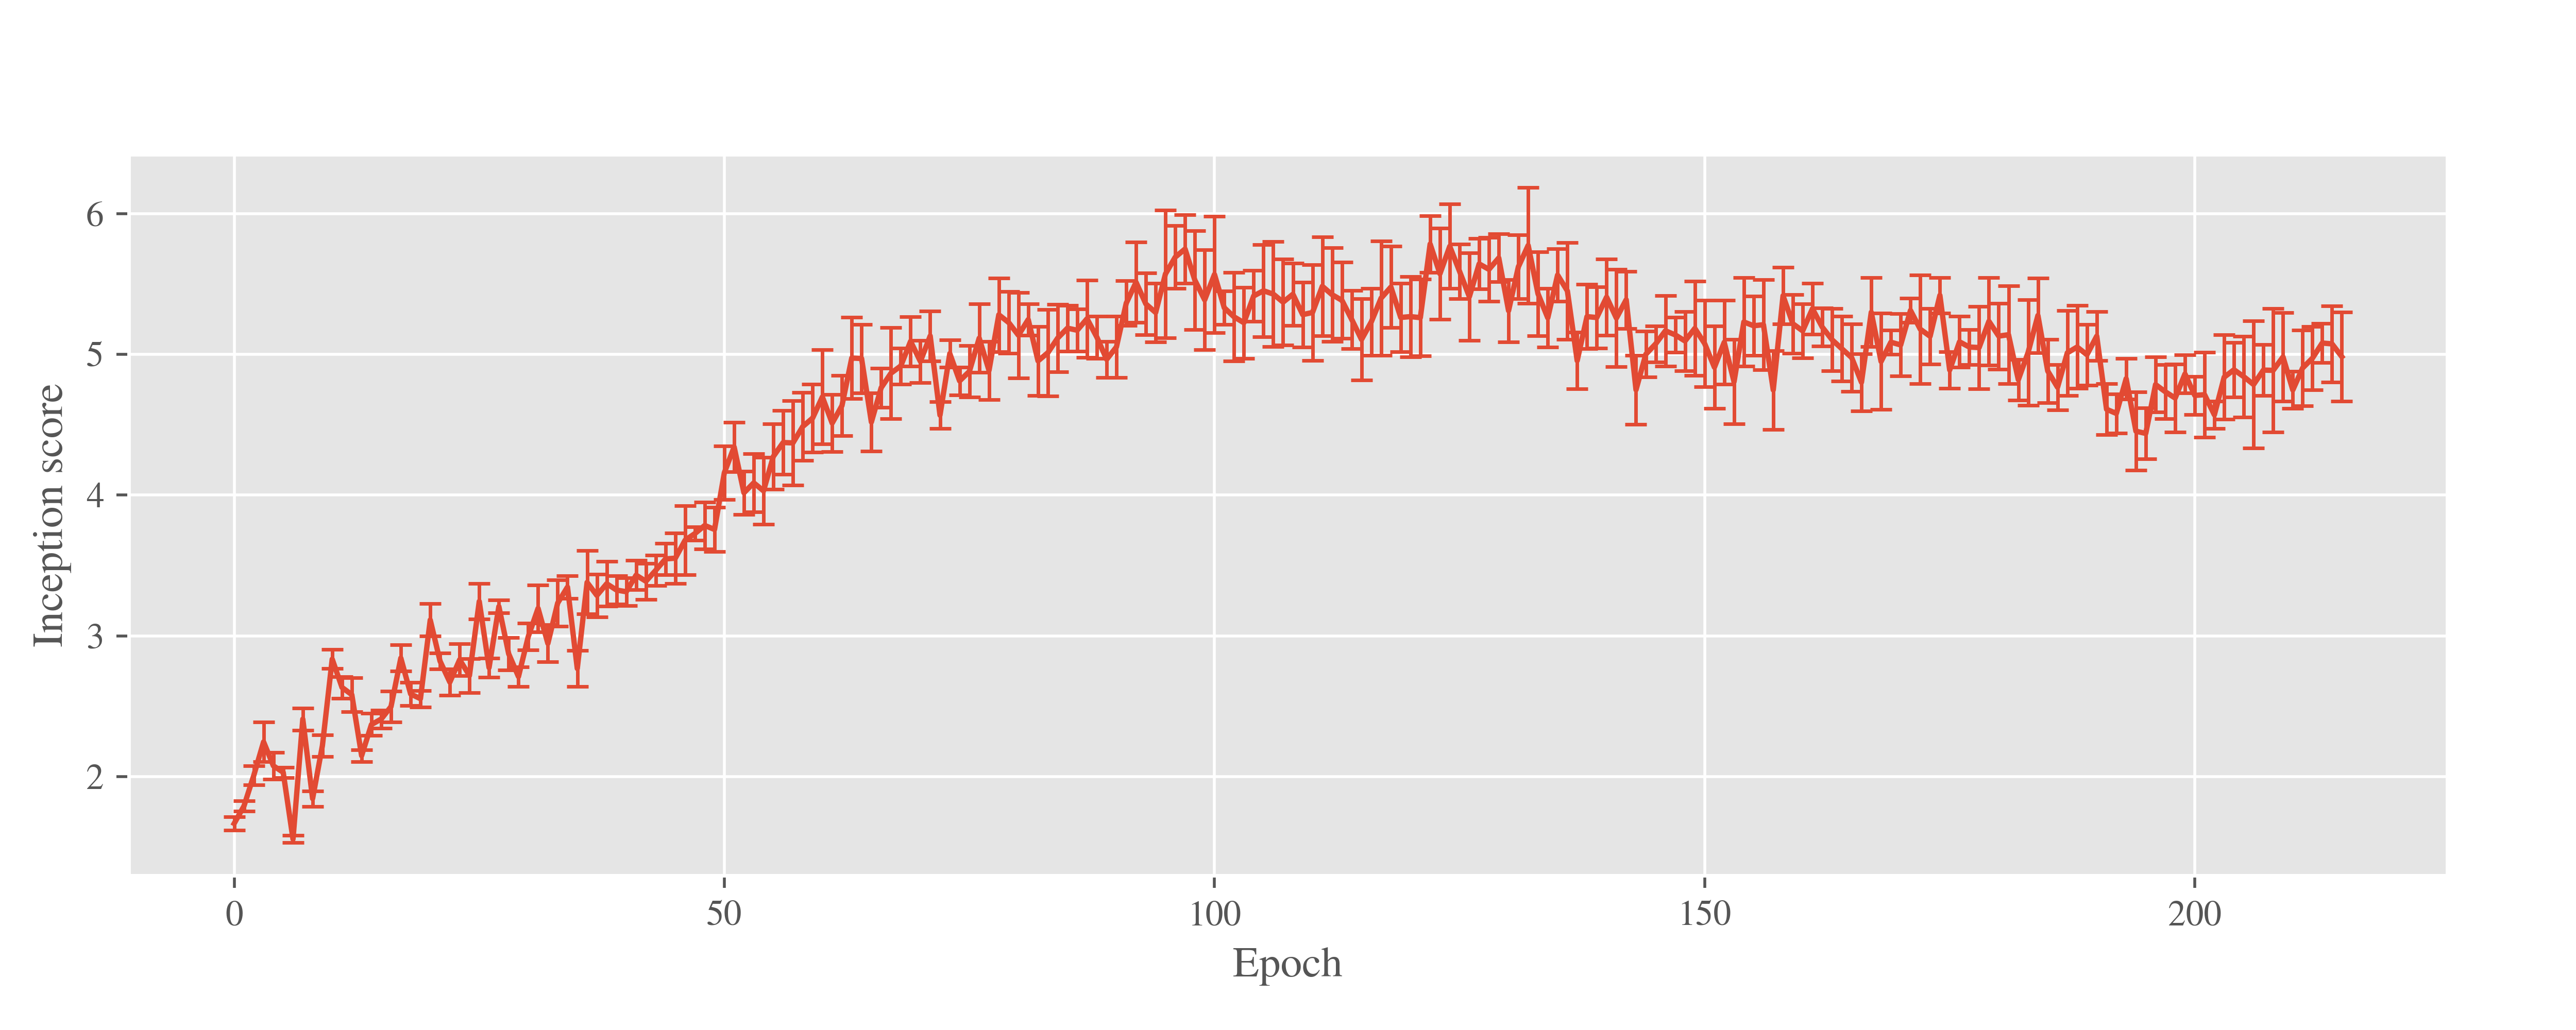
\includegraphics[width=\textwidth]{../code/results/figures/w-wc-dcgan_cifar10_is.png}
		\caption{Inception score\\~}
		\label{fig:exp-w-wc-dcgan-is}
    \end{subfigure}
    \begin{subfigure}[t]{0.49\textwidth}
        \centering
        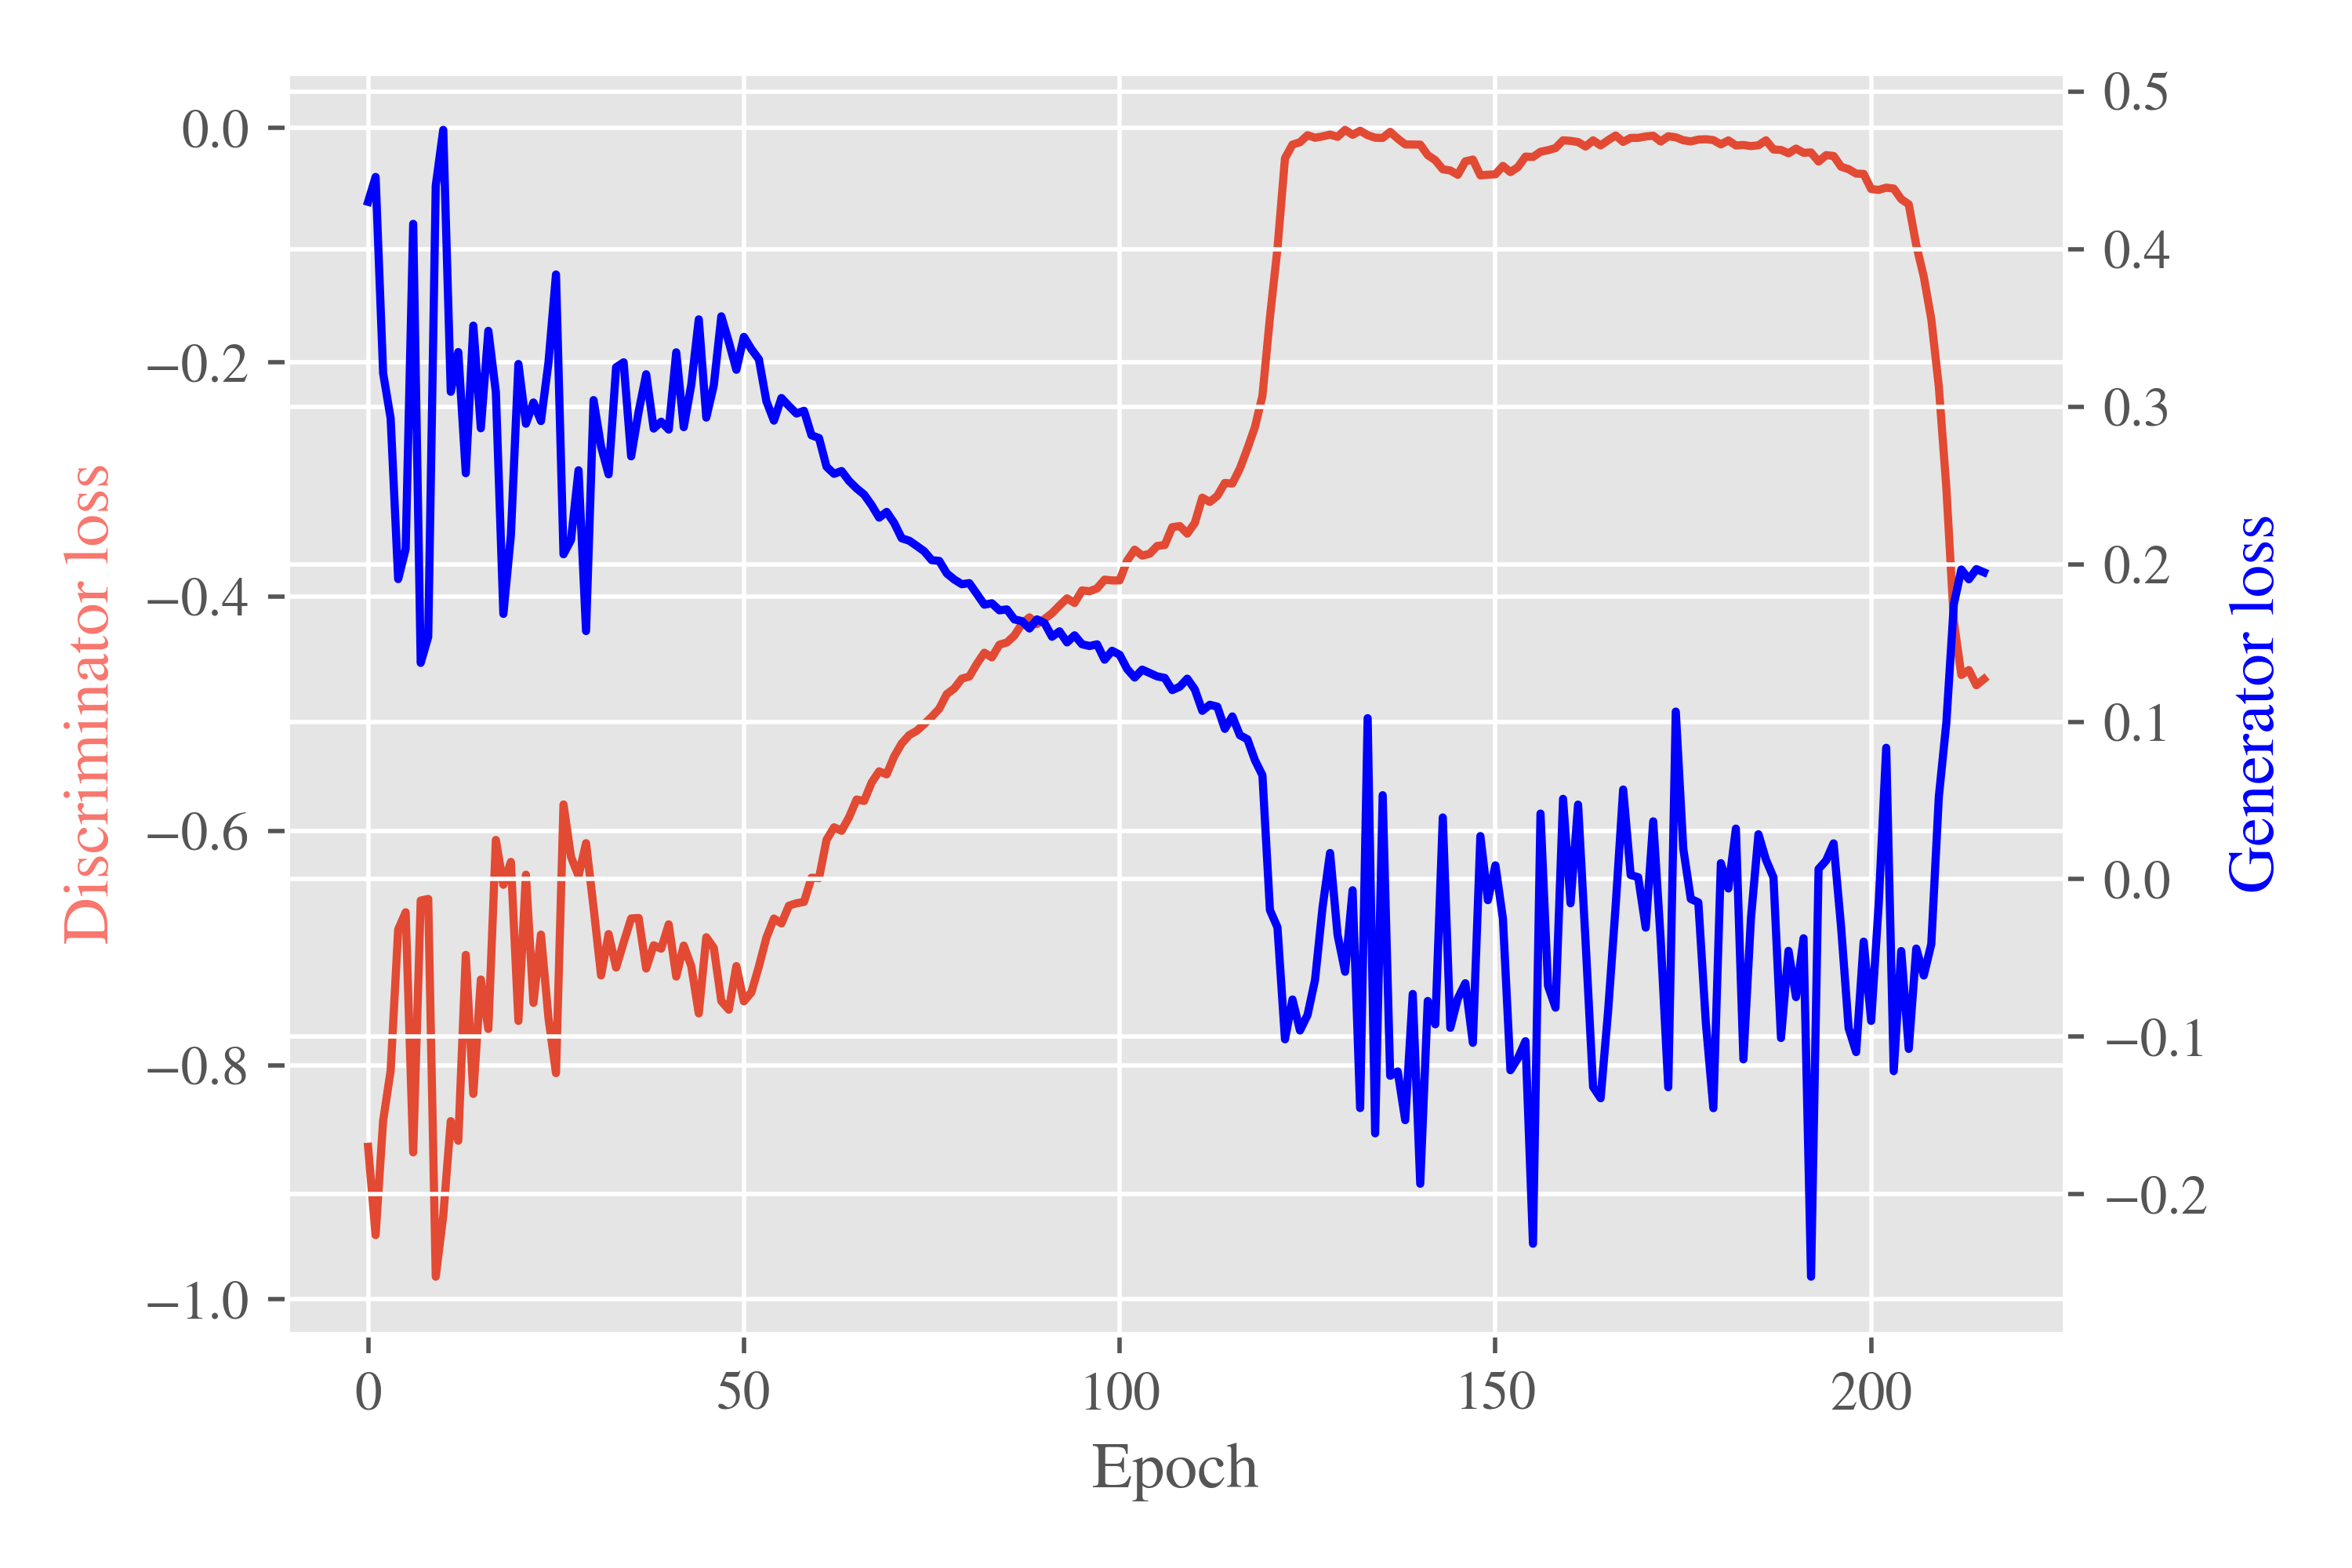
\includegraphics[width=\textwidth]{../code/results/figures/w-wc-dcgan_cifar10_losses.png}
		\caption{Losses\\~}
		\label{fig:exp-w-wc-dcgan-losses}
    \end{subfigure}
    \caption{W-WC-DCGAN - training on CIFAR10 over 200 epochs.}
\end{figure}%
We observe a turbulent climb for the Inception score and an even more chaotic evolution of the losses. Looking at the losses, it seems like the training has two different ``regimes''. We propose an interpretation, even though we cannot be sure of its accuracy. In all experiments, we initialize weights by sampling from a Normal distribution with mean 0 and standard deviation 0.02. Here, we use the recommended clipping value of 0.01 \cite{arjovsky2017wasserstein}. This means that for the first iterations, most weights are systematically clipped, and possibly by a lot. It is easy to think how this would lead to unpredictable or unstable behaviour, seemingly experienced in epochs 0 to 50. Then, we think that weights enter a range that suits the requirements of WGAN, leading to a more stable training phase until epoch 120. After this epoch, the generator seems to enter a new chaotic regime, possibly because the discriminator reached a well performing region where it becomes hard to fool. This problem might be solved with thorough hyper-parameter tuning.
\subsection{W-SN-DCGAN}
\label{sec:exp-wsndcgan}

We present the evolution of the inception score and losses in Figures \ref{fig:exp-wsndcgan-is} and \ref{fig:exp-wsndcgan-losses}, respectively.
   
\begin{figure}[t!]
    \centering
    \begin{subfigure}[t]{0.49\textwidth}
        \centering
		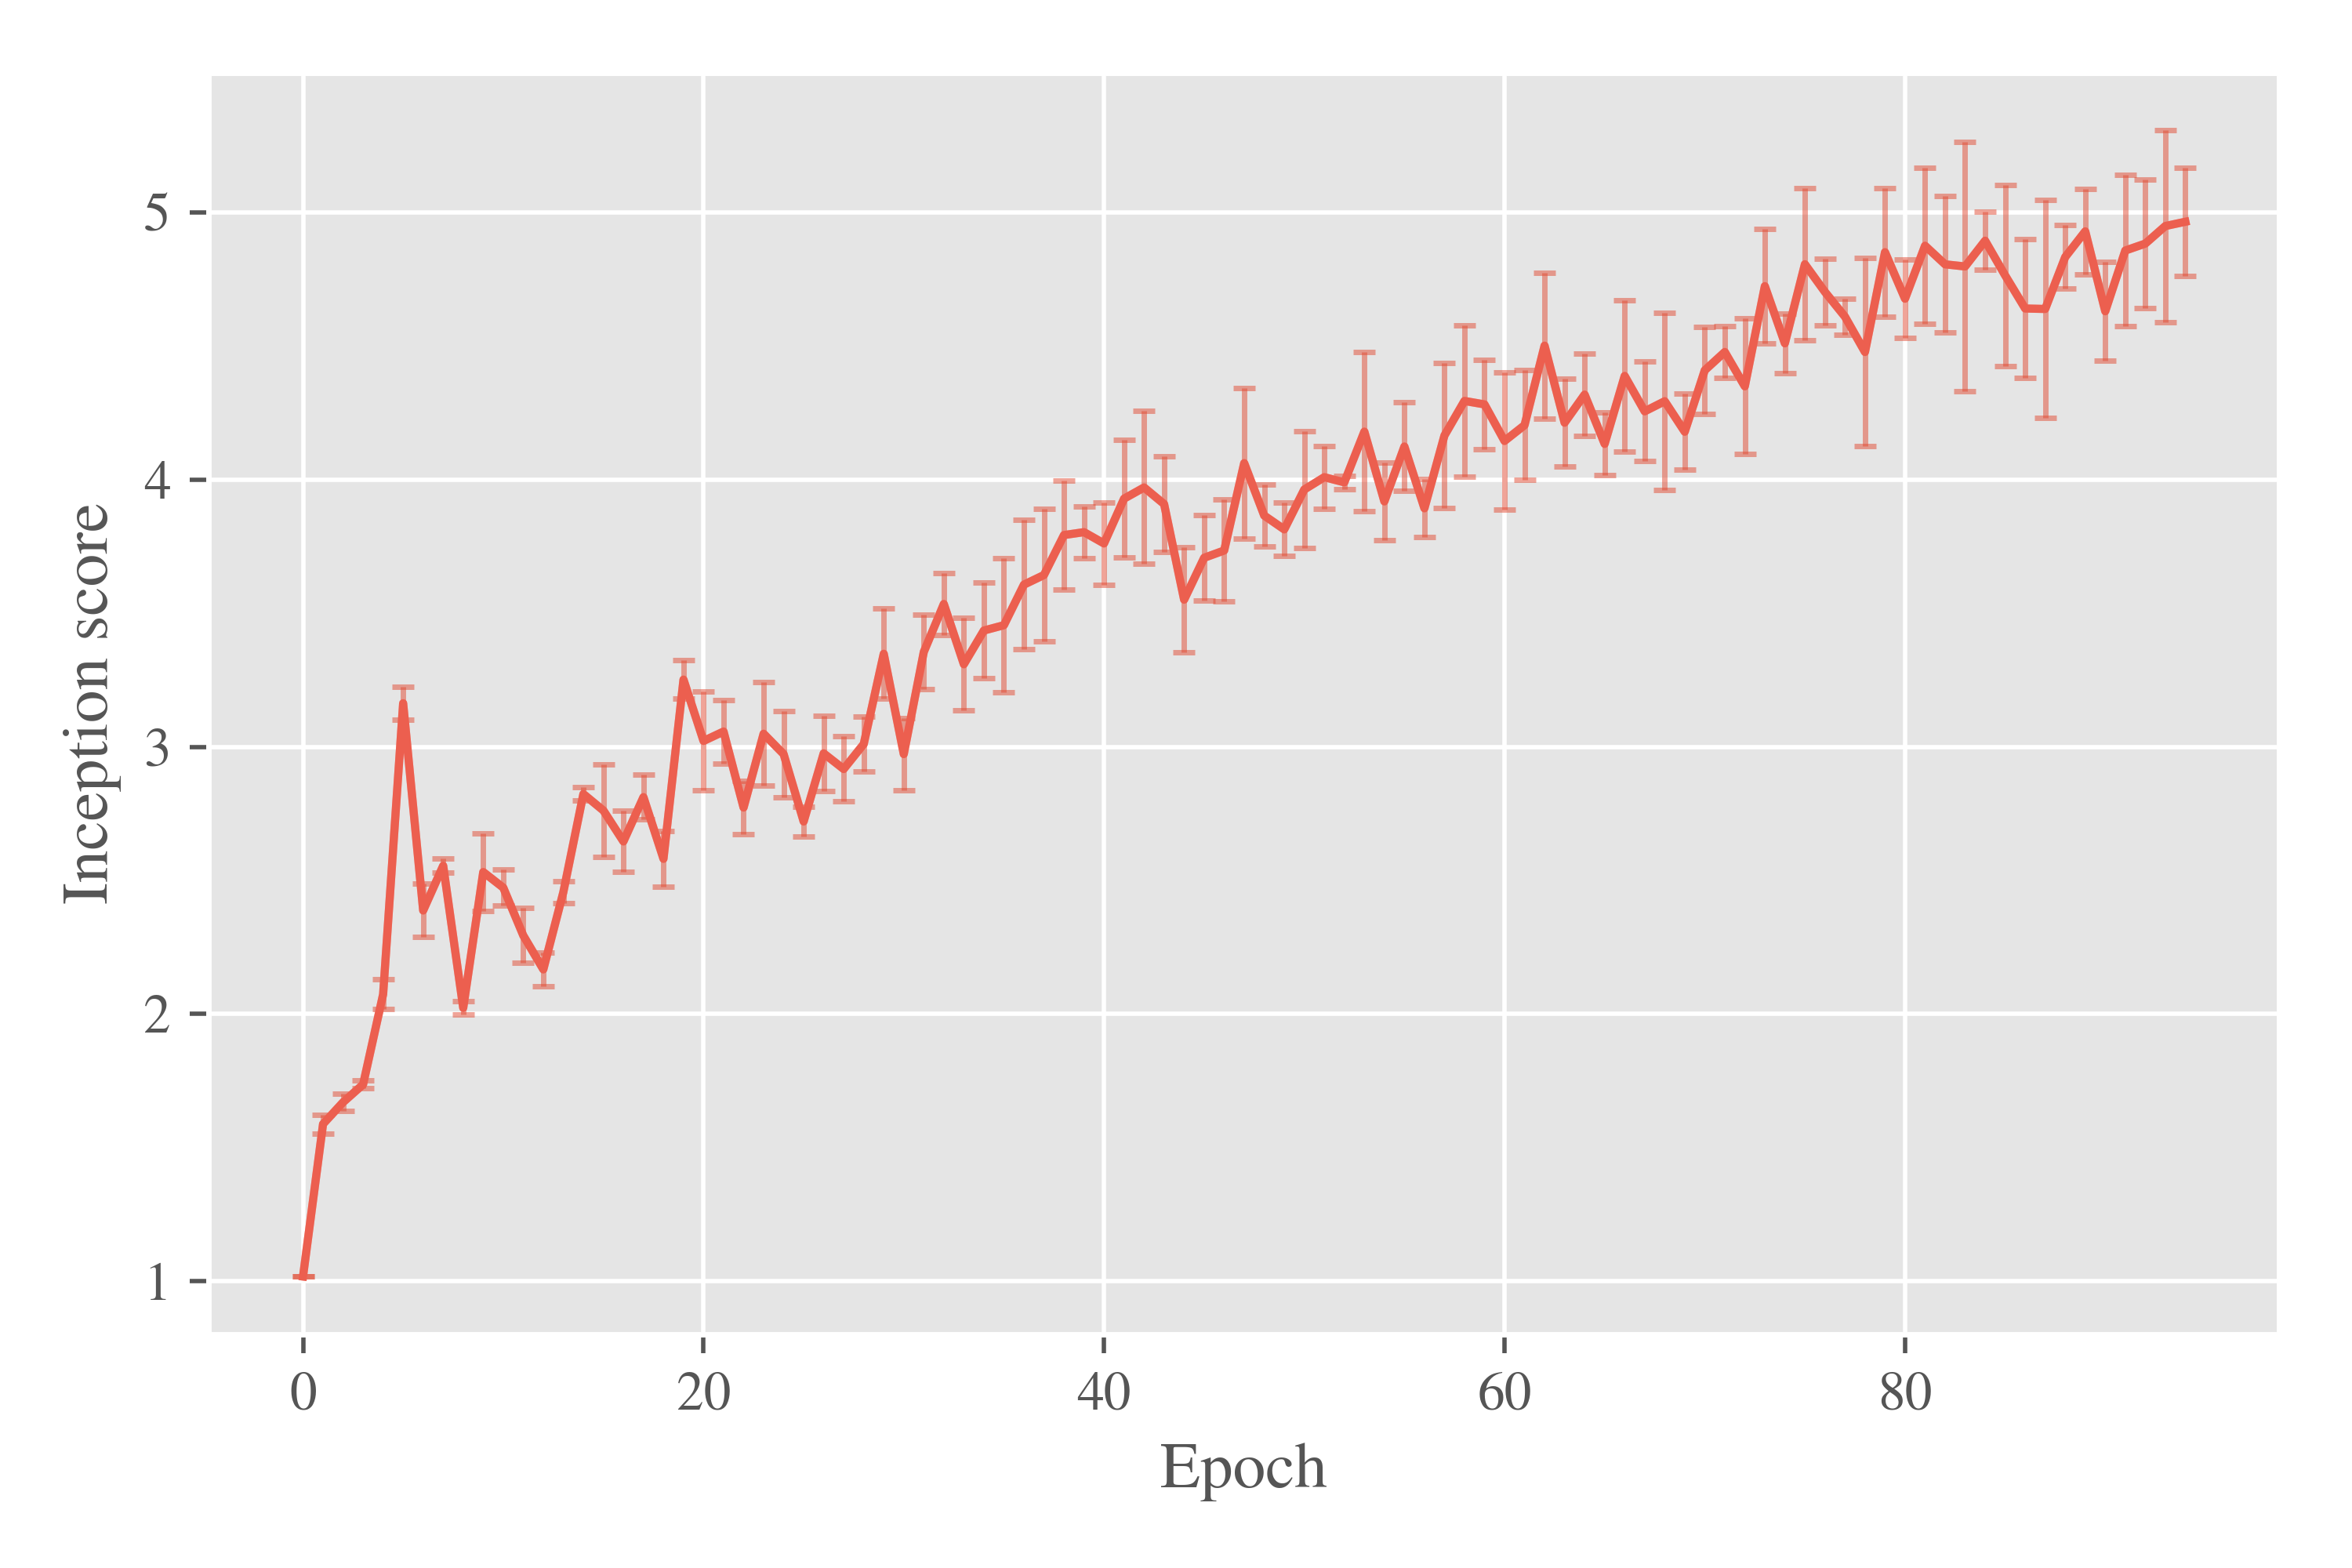
\includegraphics[width=\textwidth]{../code/results/figures/w-sn-dcgan_cifar10_is.png}
		\caption{Inception score}
		\label{fig:exp-w-sn-dcgan-is}
    \end{subfigure}
    \begin{subfigure}[t]{0.49\textwidth}
        \centering
        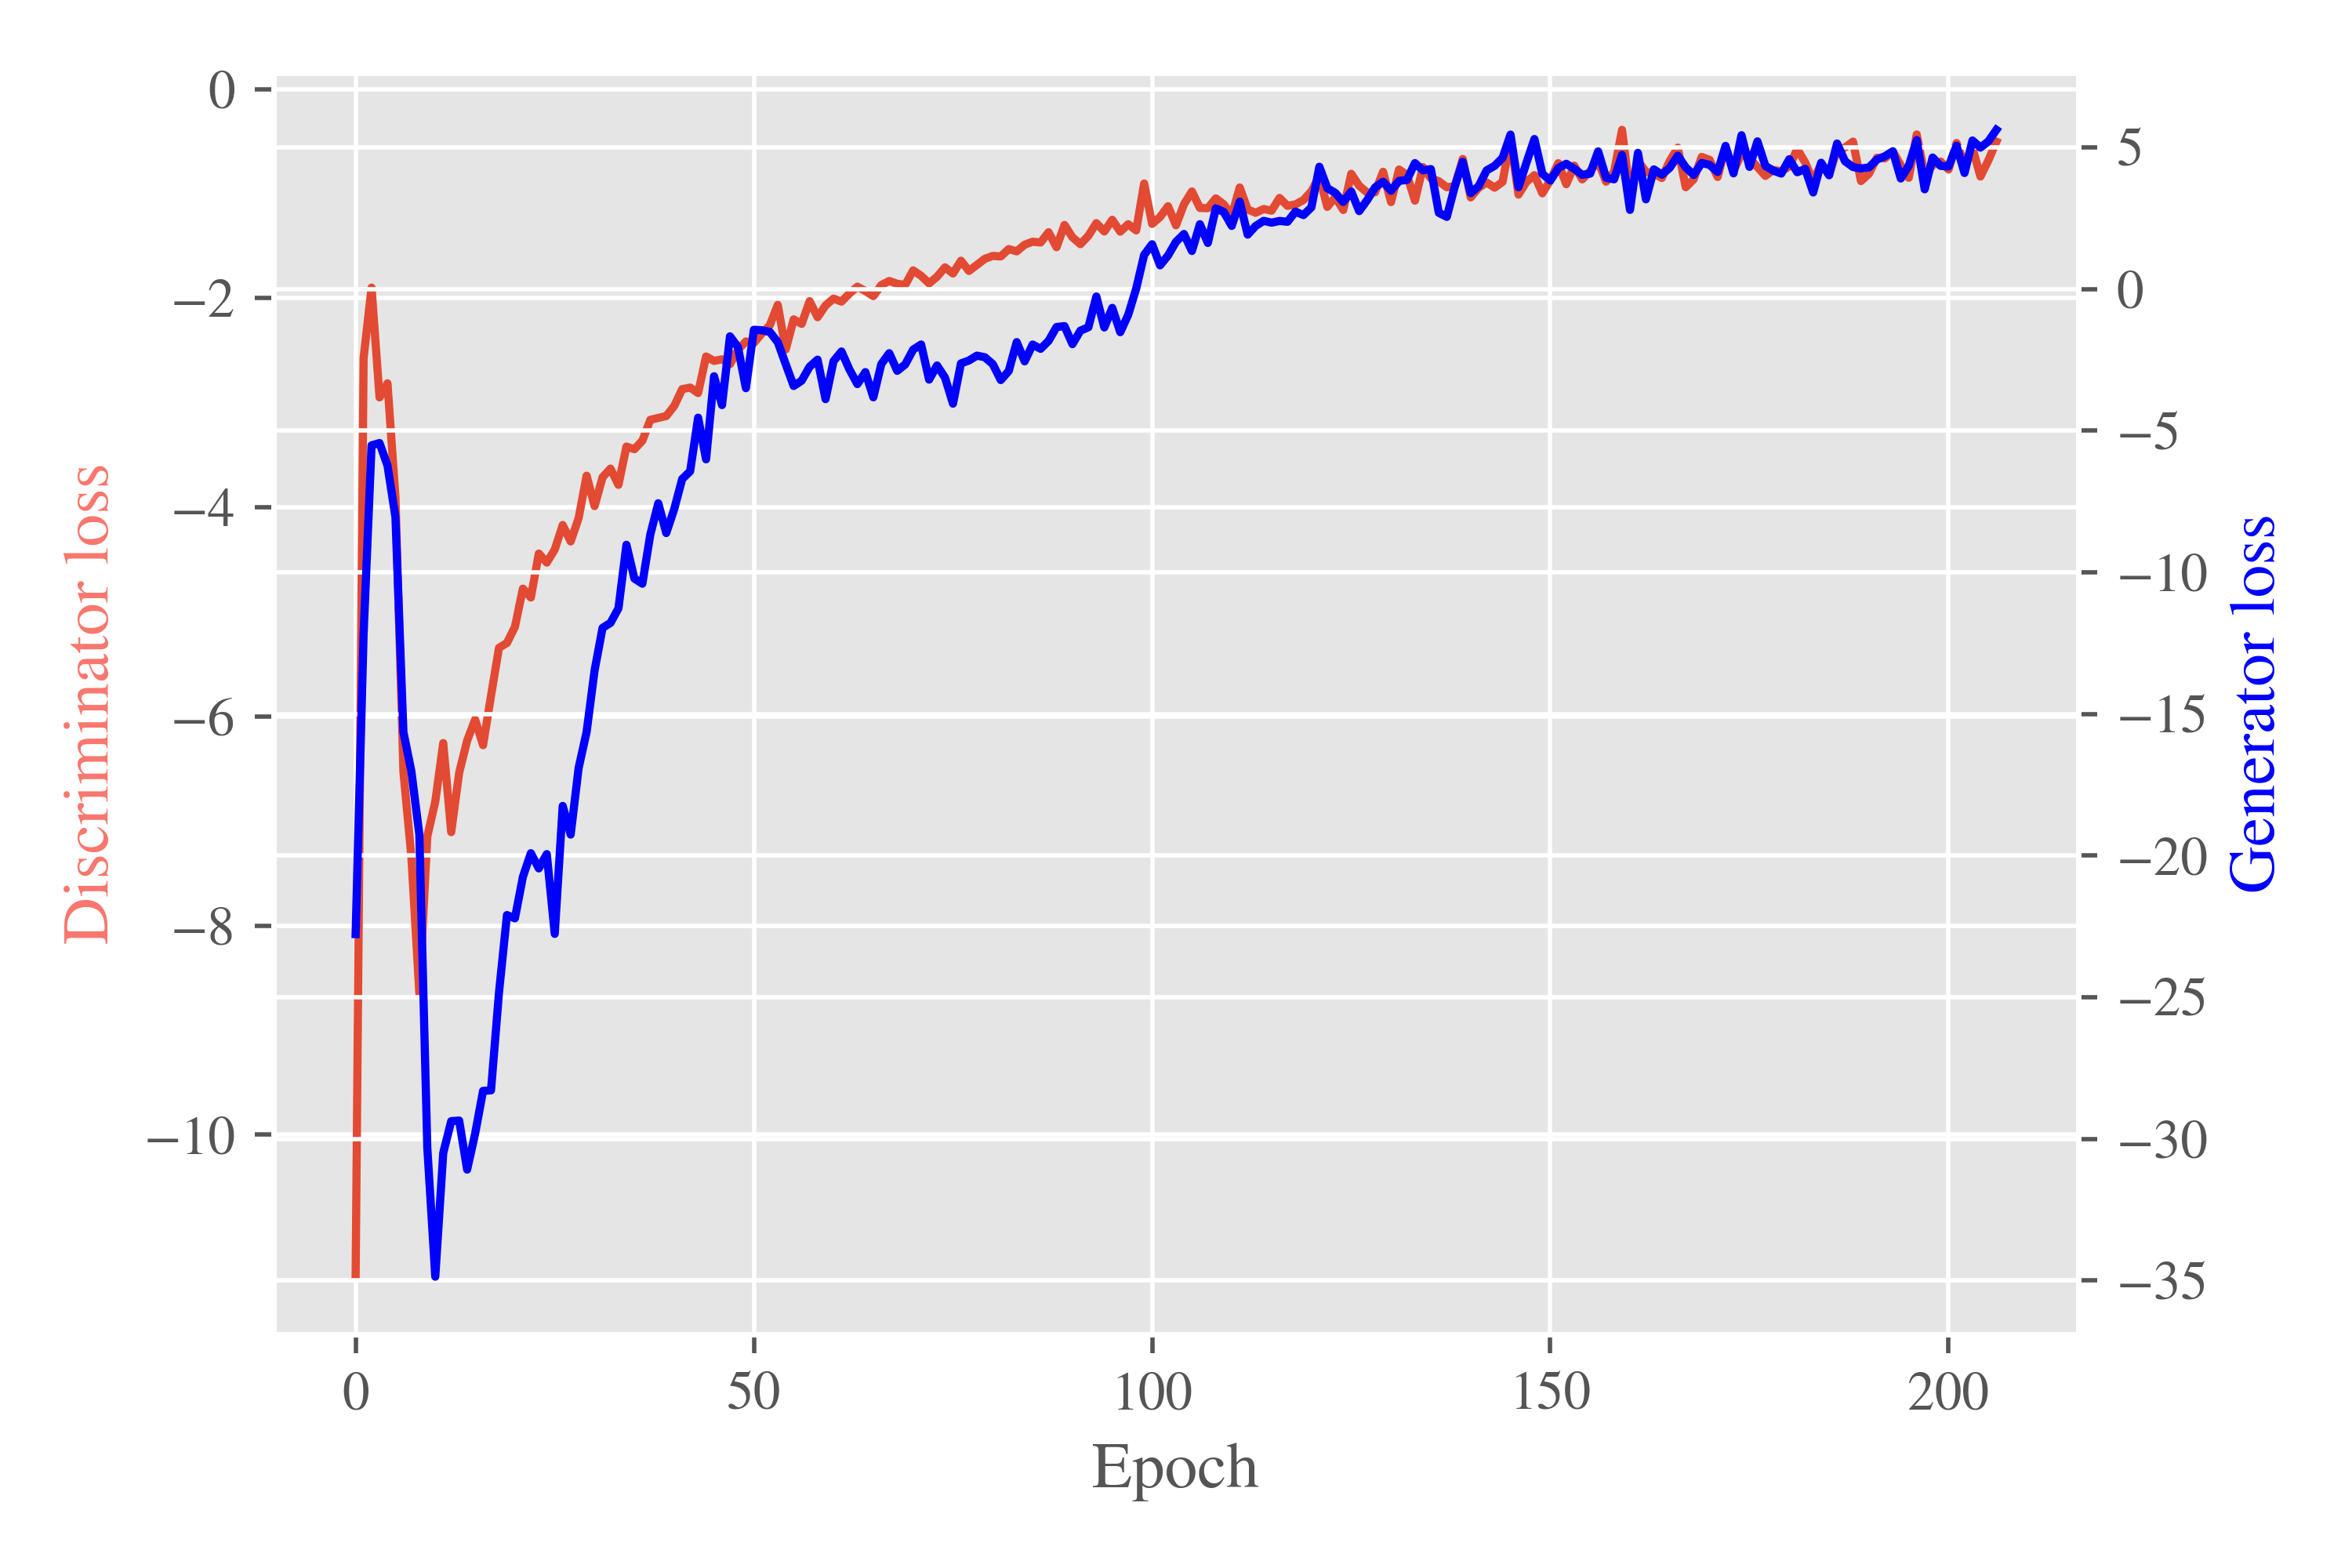
\includegraphics[width=\textwidth]{../code/results/figures/w-sn-dcgan_cifar10_losses.png}
		\caption{Losses}
		\label{fig:exp-w-sn-dcgan-losses}
    \end{subfigure}
    \caption{W-SN-DCGAN - training on CIFAR10 over 200 epochs.}
\end{figure}



\section{Conclusions}
%Explain what conclusions you can draw from these set of experiments? The set of experiments and results reported here should justify some of the design choices described in the previous sections. (3-6 pages)
\todo{to justify the use of WGAN / the need for loss smoothness: Plotting these learning curves is not only useful for debugging and hyperparameter searches, but also correlate remarkably well with the observed sample quality. (taken from WGAN paper) }

\subsection{Future Work}


- LSGAN
- Gradient penalty
- Parameter search

%
\bibliographystyle{splncs}
\bibliography{egbib}

%
~\\
\pagebreak
\appendix
\section{Template examples}

% Example table
\setlength{\tabcolsep}{4pt}
\begin{table}
\begin{center}
\caption{Font sizes of headings. Table captions should always be
positioned {\it above} the tables. The final sentence of a table
caption should end without a full stop}
\label{table:headings}
\begin{tabular}{lll}
\hline\noalign{\smallskip}
Heading level & Example & Font size and style\\
\noalign{\smallskip}
\hline
\noalign{\smallskip}
Title (centered)  & {\Large \bf Lecture Notes \dots} & 14 point, bold\\
1st-level heading & {\large \bf 1 Introduction} & 12 point, bold\\
2nd-level heading & {\bf 2.1 Printing Area} & 10 point, bold\\
3rd-level heading & {\bf Headings.} Text follows \dots & 10 point, bold
\\
4th-level heading & {\it Remark.} Text follows \dots & 10 point,
italic\\
\hline
\end{tabular}
\end{center}
\end{table}
\setlength{\tabcolsep}{1.4pt}

% Example figure
(Fig.~\ref{fig:example} shows an example).
\begin{figure}
\centering
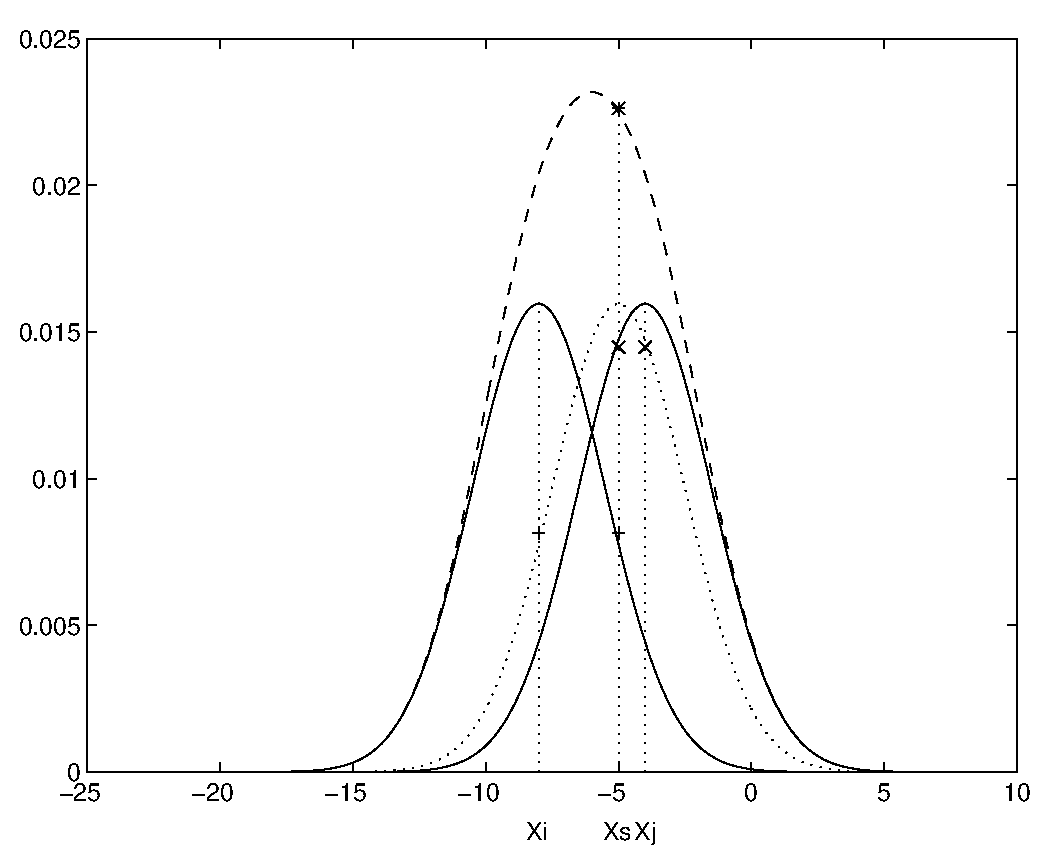
\includegraphics[height=6.5cm]{figures/eijkel2}
\caption{wuzup}
\label{fig:example}
\end{figure}

% If possible (e.g. if you use \LaTeX) please define figures as floating objects. \LaTeX\ users, please avoid using the location parameter ``h'' for ``here''. If you have to insert a pagebreak before a figure, please ensure that the previous page is completely filled.

% Example math
\begin{align}
  \psi (u) & = \int_{0}^{T} \left[\frac{1}{2}
  \left(\Lambda_{0}^{-1} u,u\right) + N^{\ast} (-u)\right] dt \; \\
& = 0 ?
\end{align}

Please punctuate a displayed equation in the same way as ordinary
text but with a small space before the end punctuation.



\end{document}
